% Paper, encoding and fonts settings
\documentclass[a4paper, openright, twoside, 12pt]{report}
\usepackage{geometry}
\usepackage[utf8]{inputenc}
\usepackage[T1]{fontenc}
\usepackage{dsfont}

% Document structure and layout
\usepackage{pdfpages}
\usepackage[toc,page]{appendix}
\usepackage{standalone}
\usepackage[absolute]{textpos}
\usepackage{setspace}
\usepackage{adjustbox}
\usepackage{rotating}

% Graphics and plotting
\usepackage{tikz}
\usepackage{pgfplots}
\usepackage{graphicx}
\graphicspath{ {graphics/} }

% Math, physics and numbers
\usepackage{amsmath}
\usepackage{siunitx}

% Extra features and enhancements
\usepackage{cite}
% Tables
\usepackage{booktabs}
% Captions
\usepackage[justification=centering]{caption}
\usepackage{subcaption}
% Listings
\usepackage{algorithm}
\usepackage{algorithmic}
\usepackage{minted}
% Make sure that hyperref is last loaded package
\usepackage[hidelinks]{hyperref}

% Pgfplots configuration
\usepgfplotslibrary{statistics}

\begin{document}
\pagenumbering{gobble}

% This page is laid out according to Silesian University of Technology's
% requirements for bachelor's thesis
\thispagestyle{empty}
\newgeometry{top=2.5cm, bottom=2.5cm, left=3cm, right=2.5cm}
% Measure absolute positioning from margins
\textblockorigin{3cm}{2.5cm}

\begin{onehalfspacing}
\begin{center}
	% Author
    \begin{textblock*}{\textwidth}(0cm, 19cm)
	\begin{flushleft}
	Autor: Maciej Ziaja \linebreak
	Promotor: dr hab. prof. Pol. Śl. Michał Kawulok \linebreak
	\end{flushleft}
	\end{textblock*}
	% Release date and place
	\begin{textblock*}{\textwidth}(0cm, 24cm)
	\fontsize{12}{12} \selectfont
	Gliwice, lipiec 2020
	\end{textblock*}
    % University logo
    \vspace{2\baselineskip}
	
\includegraphics[width=0.3 \textwidth]{polsl_logo}\\
	\vspace{2\baselineskip}
	\fontsize{18}{18} \selectfont
	% University name
	\textbf{\textsc{Politechnika Śląska \linebreak
	Wydział Automatyki, Elektroniki i~Informatyki \linebreak
	Kierunek Informatyka}} \\
	% Thesis title
	\vspace{3\baselineskip}
	Praca dyplomowa magisterska \\
	\vspace{3\baselineskip}
	\fontsize{14}{14} \selectfont
	Data augmentation for super--resolution reconstruction using deep convolutional neural networks
\end{center}
\end{onehalfspacing}
\restoregeometry


% Create minted environment for long listings with page breaks
\newenvironment{longlisting}{\captionsetup{type=listing}}{}

\cleardoublepage

% Introductory pages
\begin{abstract}
The aim of this work is to enhance super-resolution satellite imaging by using
data augmentation techniques based on deep learning algorithms.
Super-resolution is a technology that enables upscaling images to a higher
resolution with more refined details and improved quality.
Such image-enhancing techniques are nowadays undergoing rapid development
thanks to advancements in deep learning and convolutional neural networks.
Deep learning is an approach in which training data plays a key role in the
outcome and quality of the solution.
Size and quality of the dataset used to train super-resolution networks are
crucial to achieve the best results.
This is especially significant when working with satellite images, which are
effortful to acquire in large numbers.
Thus, when training a super-resolution network, it may be worth incorporating
data augmentation techniques.
Data augmentation is a process that intends to enlarge and improve training
datasets for machine learning by transforming, multiplying or generating data.
This process has been traditionally done using resampling techniques, however this work aims to use deep learning to generate datasets for training
super-resolution algorithms.
Following chapters provide an overview of modern super-resolution solutions
and a proposal of a set of deep learning algorithms to enhance the training datasets.
Results of the work are evaluated by testing super-resolution networks which
were trained on the datasets created during the project.
\end{abstract}

\tableofcontents
\cleardoublepage

\pagenumbering{arabic}

% Chapters
\chapter{Introduction}
\label{ch:introduction}
\section{Super--resolution technology}
Super resolution algorithm is a~solution that upscales images and improves
their quality.
Such an algorithm can be treated as a function that takes an image and returns
it with a resolution \textit{n} times larger.
Algorithms taken into account in the process usually upscale images two or
three times.

It is important to distinguish between super--resolution and traditional
upscaling algorithms.
The later use interpolation to enlarge images, however they hardly improve the
quality of the image.
The intent of super--resolution is not only to upscale images, but to improve
the quality and detailing.
Nowadays such an effect is achieved using machine learning, precisely---deep
learning---a technology that utilizes multi--layered neural networks trained
with large datasets.
Deep learning networks that process image data usually utilize convolutional
layers.
Such layers contain a number of image filters that are tuned during training.
Like all the rest of machine learning algorithms, the deep learning based
super--resolution works in a statistical manner.
This means that the extra details created during the image enhancement process
state an imaginary approximation of image features.

Two kinds of super--resolution algorithms can be outlined:
\textit{one--to--one} and \textit{many--to--one}.
The first one is the obvious approach, where one low resolution image is
translated into high resolution one.
The latter is more advanced technique, which utilizes multiple low resolution
images of the same scene to produce one high resolution picture.
The usual approach is to have multiple low resolution images that are slightly
shifted.
Data from these multiple images is merged together to produce image of greater
quality.
This approach can lead to best results in super--resolution, in some scenarios
the data fusion can lead to recreation of high resolution details, that are
hardly visible in any single low resolution image.
It should be noticed that the super--resolution networks trained on
domain--specific data often cannot be used to enhance images with different
contents.
For example, if a network was trained on a dataset with human faces it is
likely to perform poorly on satellite images.
Network architecture can also be domain--specific, for example utilizing
different bands of a multispectral image.

Super--resolution is a technique relevant in the field of satellite imaging and
geoscience.
The most common reason for image enhancement is for aesthetic reasons.
This application is viable in satellite imaging, however super--resolution can
lead to other practical advantages.
Image enhancing techniques can be used as a preprocessing step in remote
sensing pipelines.
For this reason super--resolution can be especially useful when considered in
the context of satellite imagery.

\section{Purpose of data augmentation and available solutions}
Deep learning, utilized in the modern super--resolution techniques, requires a
lot of data to train successfully.
Increase in quality and size of dataset can lead to far better results when
training a neural network.
This is why data augmentation techniques are often used to improve performance
of deep networks.
Data augmentation incorporates various transformation to improve, multiply or
generate training data.
Common techniques to improve image data include: zooming, resizing, shifting,
flipping, rotating, distorting, adding noise, modifying colors and exposure.
These operations may be application--specific.
To give an example, one should beware distorting or flipping data containing
with constrained geometry, like road signs.
The mentioned augmentation techniques can be considered classic and rather
trivial.
However more advanced approach can be taken to generate data.
It is possible to create deep neural networks to create data augmentation
transformations.
This approach can be especially useful when a dataset is available, that it is
too small to train the desired network.
A smaller network can be made and trained on existing small dataset to multiply
the data.
Then the augmentation network can be used to generate more data for the
original model to learn.
With deep learning capabilities networks can learn to multiply, transform or
even generate data without direct input.

\section{Aim of the work and motivation}
The objective of the work is to create a set of augmentation networks for
enhancing super--resolution training data.
Subsequent chapters will present considered super--resolution architectures
with greater details and propose neural network models for data augmentation.

The nature of super--resolution technology and satellite imagery impose certain
ways in which data augmentation should be applied to the training data.
Super--resolution is trained using pairs of data---low resolution image with
high resolution image (or a set of low resolution images with high resolution
image in case of many--to--one network).
This requirement renders compiling training sets a challenge, especially in the
field of satellite imagery.
In such scenario the most common technique is to use resizing algorithms on
single image datasets.
A set of training pairs can be created by downscaling high--resolution images.
In the case of many--to--one networks, single high--resolution image can be
multiplied and shifted before shrinking to create more low--resolution images.
Such technique may work well, however it infuses the data with information
about resizing algorithms.
The way high--resolution and low--resolution images relate in such a set
depends heavily on the interpolation algorithm (e.g. bicubic, bilinear,
nearest, lanczos).
Network trained on such datasets will likely learn to invert given
interpolation methods.
This does not match exactly real--life scenarios, most images are not created
using resizing algorithms.
Another approach, utilizes pairs of real low--resolution and high--resolution
images of the same scene, taken by cameras of different quality.
The con of this method is challenging data acquisition process---satellite
images are rarely taken in pairs.
Such a dataset has to be deliberately made with super--resolution in mind,
which makes such data less common.
The main idea of the project is to use such a dataset of real--life data to
train an augmentation network.
Such a network would learn to create low--resolution images for
high--resolution, without imprinting resampling algorithms mechanisms into the
data.
The relation between low and high--resolution images in such an augmented
dataset would resemble relation between same image taken by cameras of
different quality. 
The augmentation neural network can be then used on other satellite image
datasets to generate training data pairs for super--resolution.
Different data, models and generation techniques can be used to achieve desired
results.
Possible variations are discussed in the course of this work to improve
super--resolution datasets.


\chapter{Analysis of related work}
\label{ch:analysis}
This chapter provides an overview and analysis of related works.
Subsequent sections introduce characteristics of satellite imagery, discuss topics of deep learning and super-resolution.
Following part of the work provides theoretical grounding for techniques used in the latter Chapters \ref{ch:scope}, \ref{ch:augmentation} and \ref{ch:sr-evaluation}.

\section{Overview of super-resolution techniques}
As mentioned in Chapter \ref{ch:introduction} super-resolution techniques can be divided into single and multi-image categories where one or many low resolution images are turned into a high-resolution one.
The latter is more advanced technique, which utilizes multiple low-resolution
images of the same scene to produce one high resolution picture.
The usual approach is to utilize multiple low--resolution images that are slightly shifted (in subpixel domain).
Data from these multiple images is merged together to produce an image of greater quality \cite{kawulok-2019-multisr}.
This approach can lead to best results in super--resolution.
In some scenarios the data fusion can lead to recreation of high resolution details that are hardly visible in any single low--resolution image.
In the case of multi-image super-resolution, better image quality comes at a cost of obtaining a series of input pictures instead of one, as it is in the single-image approach.

The simplest super-resolution approach predates deep-learning techniques and utilizes interpolation techniques for multi-image data.
Multiple low-resolution images with subdomain shifts can be used to achieve more detailed interpolation for missing values in the reconstructed high-resolution picture \cite{park-2003-sr}.
Nowadays super-resolution is mainly done with deep learning techniques which undergo a rapid development.
Deep learning based super-resolution can be divided in regard to: supervision (supervised or unsupervised learning), application domain, network architecture, learning strategy and evaluation technique \cite{wang-2019-srsurvey, bashir-2021-srreview}.

\section{Characteristics of satellite imagery}
This work centers around super--resolution technique in the sphere of satellite imagery.
As mentioned in the introduction (Chapter \ref{ch:introduction}), image enhancing can be domain-specific.
This is especially crucial when satellite photos are taken into account.
Pictures taken from aerospace devices differ substantially from normal photography.
Multi-image observation is usually favoured over single--image.
Satellites often take a series of photos of a single scene.
This puts emphasis on the multi image super--resolution techniques in the many--to--one fashion.

Another unique feature of satellite observations is the usual spectral width of the imagery.
Scientific \textit{hyper--spectral} apparatus present on satellites often take photos in a very wide spectrum that may not include frequencies of visible light.
This specific kind of image with large spectral dimension is often called a \textit{hyper--spectral cube}, because it can be represented as a three--dimensional tensor (cube) with height, width and spectral dimensions.
Spectral bands in the cube have the same width and sample adjacent parts of spectral range.
The \textit{multi-spectral} devices take pictures in multiple different bands of different wavelenghts.
Spectral bands in a multi-spectral image can contain wavelengths such as infrared, near--infrared, panchromatic\footnote{A spectral range similar to the range of traditional monochromatic grayscale photography. This range is usually highlighted because of connections with pre--digital imaging of the past century.}, radio frequencies and more.
Such images are often stored in special file formats or in a series of high bit--depth standard lossless image formats, such as PNG or TIFF.
These can take up to 13 bands  or more in different files per a single satellite photography.

One more crucial property of satellite imagery is the GSD (\textit{ground sample distance}) parameter, which denotes spatial distance between pixels of a digital image.
For example, one--meter GSD states that that location of adjacent pixels is one meter apart on the ground.
The GSD parameter determines size of objects visible in the satellite pictures.

Super-resolution for satellite imagery has been developing rapidly in recent years.
The growth of this field was accelerated by Proba-V super-resolution competition organized by the European Space Agency \cite{esa-proba-competition} .
The challenge lasted from the end of 2018 to June of 2019 (over half a year).
Architectures submitted in the competition have pushed super-resolution beyond previous baseline performance scores.
A more detailed description of the Proba dataset can be found in Section \ref{sec:probav}.

\section{Machine learning for image processing}
Both the augmentation process and the super-resolution implementations in this work are baed on machine learning---especially deep learning.
Following chapters provide an overview of these methods for image processing.

\subsection{Neural networks and deep learning}
\textit{Machine learning} is a computer science technique that solves problems by fitting algorithms to data, by optimization algorithms and statistics.
This approach contrasts with the traditional imperative problem--solving, where algorithms are designed with step--by--step attitude.
\textit{Artificial neural networks} are machine learning structures modeled after living organisms and structure of brain.
The traditional neural networks consist of layers of densely connected neurons.
Each of the neurons contains a set of inputs with connected weights.
The output of a neuron is passed through a nonlinear activation function.

Training a neural network in a supervised manner requires a set of examples bounded with ground truth labels.
The fitting process of such a network consists in adjusting the input weights.
Learning is done in steps called \textit{epochs}, during each epoch the training set is passed through the network.
The output of the network is then compared with the ground truth labels.
This is done according to a given \textit{loss function} which serves as a metric between the actual and expected output of the network.
Then the loss is used to optimize the wights via \textit{gradient descent} methods.
The gradients are computed using \textit{backpropagation} algorithm which is based on the chain rule of derivatives.
There are various loss functions and optimizers to choose from and apply according to the given problem.
In modern deep learning datasets may be too big to apply backpropagation in one pass.
For this reason, weights are usually updated using small subsets called \textit{batches}.

This kind of machine learning architecture has been initially used with manual feature extraction.
Utilization of a set of predefined convolutional filters may be an example of this approach in the domain of image processing.
A set of such filters would include basic geometric shapes.
These small filters would be convolved with the input image.
The results of such an operation would be then fed into the neural network to get the final result of image processing.
With the advancements in the machine learning area, a new kind of neural network layer was created---a \textit{convolutional layer}.
These layers consist of (one, two or even three dimensional) filters that can be convolved with the input image.
However, in  contrast to the manual feature extraction technique, these filters are adjusted in the fitting process of the network.
Elements in the filter tensor are treated like neuron weights, and they are accommodated during gradient descent.
This enables creation of much better perfoming and flexible image processing neural networks.
Convolutional layers can also be viewed as a dense layer with shared weights between groups of pixels.
This way, every pixel can be used in the fitting process without connecting every value in the image, which would result in very big and hard-to-train networks.

However, the creation of convolutional neural networks leads to increasing complexity and number of parameters in models.
This issue can be addressed by using very large datasets for the fitting process.
Nowadays, the smallest datasets for training modern neural networks contain thousands of images.
Such trainings require a lot of time and processing power; they usually must be performed using (even multiple) GPUs and may last a few days.
This combination of three factors: complex multi--layered neural networks (often with media--oriented specialized layers), very large datasets (often with many classes and objects) and utilization of expensive time and resource--consuming trainings constitute what is called \textit{deep learning}.
This kind of machine learning has proven, in the last ten years, to hold a revolutionary potential, pushing forward techniques such as image and audio processing beyond what is possible with older methods.
Modern super--resolution, which this work revolves around, is possible thanks to advancements in the deep learning.

\subsection{Encoder--decoder mechanism}
Encoder--decoder network architecture is a common pattern in generative image processing.
It is used both in data augmentation networks presented and super-resolution model utilized in Chapters \ref{ch:augmentation} and \ref{ch:sr-evaluation}.
Encoder--decoder translates input data into abstract state during encoding, then reconstructs it when decoding.
The mid--point of the architecture usually bottlenecks the information containing compressed--like data.
Convolutional interpretation of the encoder--decoder is usually used when working with images.
During the encoding process the depth of input is usually increased and spatial dimensions are shrunken.
This is achieved by subsequent usage of convolutional and pooling layers.
After encoding, the compressed data can undergo some form of processing.
For example, it can be flattened and passed through a densely connected layer, although this is rarely applied in the super--resolution, because fully--connected layers break the fully convolutional nature of a network (meaning that it cannot process images of varying spatial size).
The decoding process commonly reconstructs depth dimensions into spatial size by upsampling or transposed convolution.
The output may match the input dimension; however, it is not necessary.
In super--resolution it is common to output data of different size than the input.
Encoder--decoder architecture is appropriate for image--to--image transformations in machine learning.
The inner workings of such an architecture are shown in the figure \ref{fig:encoder-decoder}, where $ x $ and $ y $ denote input and output and $ z $ is the encoded hidden state. 
\begin{figure}
    \centering
    \documentclass[tikz]{standalone}
\usepackage[utf8]{inputenc}

\usetikzlibrary{positioning}
\usetikzlibrary{shapes.geometric}

\begin{document}
	
\tikzset{arrow/.style={-stealth}}

\begin{tikzpicture}
	\node[fill=blue!20, minimum width=0.5cm, minimum height=3.5cm] (X) at (0,0) {$\mathbf x$};
	
	\draw([xshift=0.5cm]X.north east) -- ([xshift=2.5cm,yshift=0.5cm]X.east) -- ([xshift=2.5cm,yshift=-0.5cm]X.east) -- ([xshift=0.5cm]X.south east) -- cycle; 
	\node at (1.75,0) {\textsc{Encoder}};
	
	\node[fill=blue!20, minimum width=0.5cm, minimum height=1.0cm] (Z) at (3.5cm,0) {$\mathbf z$};
	
	\draw([xshift=0.5cm]Z.north east) -- ([xshift=2.5cm,yshift=1.25cm]Z.north east) -- ([xshift=2.5cm,yshift=-1.25cm]Z.south east) -- ([xshift=0.5cm]Z.south east) -- cycle;
	\node at (5.25,0) {\textsc{Decoder}};
	
	\node[fill=blue!20, minimum width=0.5cm, minimum height=3.5cm] (Xp) at (7,0) {$\mathbf y$};
	
	\draw[arrow] (X.east) -- ([xshift=0.5cm]X.east);
	\draw[arrow] ([xshift=-0.5cm]Z.west) -- (Z.west);
	\draw[arrow] (Z.east) -- ([xshift=0.5cm]Z.east);
	\draw[arrow] ([xshift=-0.5cm]Xp.west) -- (Xp.west);
\end{tikzpicture}
\end{document}
    \caption{Schematic of encoder--decoder mechanism}
    \label{fig:encoder-decoder}
\end{figure}

Encoder--decoder mechanism is often enhanced with \textit{residual connections}.
These are often called \textit{skip connections} because they form parallel branches in networks that skip certain operations.
These skip routes are then summed with the result of an operation, resulting in additional direct flow of information during forward and direct gradient flow on the backward pass.
Residual connections applied between arms of an encoder--decoder create what is called \textit{U--Net} architecture.
In the case of super--resolution processing, the forward skips can be viewed as routes for transporting unprocessed low--frequency information.
This information can be used during the decoding step in the encoder--decoder scheme.

\subsection{Generative Adversarial Networks}
\label{sec:gans-overview}
In recent years, a new approach to training generative neural networks has emerged.
The traditional supervised learning described in the previous sections consists in providing the network with an input and comparing the generated output with a ground truth to compute loss.
The \textsc{gan}---\textit{generative adversarial network} approach requires creating two networks, a \textit{generator} and \textit{discriminator} \cite{goodfellow-2014-gans}.
The former is tasked with generating data, while the latter learns to differentiate images created by the generator from real ones.
In the \textsc{gan} scheme the discriminator learns like a traditional binary classifier---it is provided with real and generated images, which are labeled accordingly.
Then discriminator loss is computed using standard classification metrics like \textit{binary cross--entropy}.
However, the generator learns in a more unique way; it creates an output image that is fed into a discriminator.
The generator loss is calculated depending on how well it produces data that may be classified as \textit{real} by a discriminator.
If the generated image is recognized as a \textit{fake} one, it receives a big penalty in the form of a large loss.
The inner-workings of a \textsc{gan} network can be visualized in the form of a graph, as in the figure \ref{fig:gan-training}.
\begin{figure}
    \centering
    \documentclass[tikz]{standalone}
\usepackage[utf8]{inputenc}

\usetikzlibrary{positioning}
\usetikzlibrary{shapes}
\usetikzlibrary{calc}

\begin{document}
	
\tikzset{arrow/.style={-stealth}}

\begin{tikzpicture}[ampersand replacement=\&]
   	\node[text width=0.25cm] at (-2.5,0) (X) {$ \mathbf x $};		 
    \node[rectangle, rounded corners, draw, fill=blue!20, minimum height=1cm] at (0,0) (G) {\textsc{Generator}};	
    \node[rectangle, rounded corners, draw, minimum height=1cm] at (3,0) (S1) {\textsc{Sample}};
    
    \node[text width=0.5cm] at (0.75,3) (Y) {$ \mathbf y_{gt} $};		 
    \node[rectangle, rounded corners, draw, minimum height=1cm] at (3,3) (S2) {\textsc{Sample}};
    
    \node[rectangle, rounded corners, draw, fill=blue!20, minimum height=1cm] at (6,1.5) (D) {\textsc{Discriminator}};
    
    \node[text width=2cm] at (10,1.5) (O) {\textsc{Real/Fake Prediction}};
     
    \path[arrow] (X) edge (G)
    (G) edge (S1)
    (S1) edge (D.south west)
    (Y) edge (S2)
    (S2) edge (D.north west)  
    (D) edge (O)
    ;
\end{tikzpicture}

\end{document}
    \caption{Schematic of \textsc{gan} network inner--workings}
    \label{fig:gan-training}
\end{figure}

\textsc{Gan}s can have many variations, the most common type utilizes unsupervised or semi--supervised data generation.
This means that in many GANs the generator can be fed with values from proper random distribution (often called \textit{latent space}) to generate new data.
An ability to create images without direct input is a great advantage of adversarial networks.

In general, adversarial network architectures provide great generative capabilities.
For this reason, GANs are widely used for data augmentation and creation \cite{bulat-2018-supergan, sundaram-2021-gangen, shorten-2019-augmentation, perez-2017-augmentation}.
A variant of GAN architecture is later used in this work for creating super-resolution training data in Chapter \ref{ch:augmentation}.

\subsection{Measuring quality of image--generating neural networks}

Both super--resolution networks and data augmentation networks input and output images.
Quantitive evaluation of such networks require comparison of two images---the network output and the ground truth reference image.
Images are usually compared using metrics like \textit{mean absolute error}, \textit{mean square error} and \textit{peak signal to noise ratio (PSNR)}.
These calculate error between pairs of corresponding pixels in different ways.
However, these metrics may be insufficient for super--resolution related problems.
Calculating pixel--wise differences does not resemble the way humans estimate image quality.
Images of varying perceived quality can have the same \textit{PSNRs} compared to the reference image.

To measure image similarity in a more reliable way \textit{structural similarity index (SSIM)} \cite{wang-2004-ssim} was introduced.
\textit{SSIM} calculates image quality in three main components:
\begin{itemize}
	\item Average \textit{luminance}.
	\item \textit{Contrast} as standard deviation of pixels.
	\item \textit{Structure} as luminance difference divided by standard deviation.
\end{itemize}
However, these values are not calculated globally.
Instead, \textit{SSIM} values are measured using windows with pixel weights determined by Gaussian distribution.
Values of \textit{SSIM} components are combined using a compound formula.
The precise mathematical description of the SSIM metric can be found in the bibliography.
Advantages of \textit{structural similarity index} render it suitable for super--resolution related image quality evaluation.

However, modified versions of the previously mentioned traditional metrics can also prove to be useful in the image comparison, one of them being the \textit{cPSNR}.
The traditional PSNR has a potential drawback of being sensitive to bias in image brightness.
This metric equalizes average brightness of compared images before calculating standard PSNR to alleviate this problem.
The improved version of PSNR was introduced and used for scoring in the Proba-V super-resolution competition \cite{esa-proba-competition}.
Various of the mentioned metrics were in this work, in accord to specific requirements of each step in the augmentation and super--resolution training process.

\subsection{Image registration}
\label{sec:registration}
Another challenge often encountered during super--resolution training and evaluation consists in aligning image pairs correctly.
Often two images that are to be compared are slightly shifted; it is common for these dislocations to lie in sub--pixel domain.
The process of aligning two similar images is called \textit{image registration}.
Registration can be performed either with traditional or deep learning-based algorithms.
To register the sub--pixel translations, images can be upscaled before using a matching algorithm.

Registration algorithms can be divided by the applied methodology of image processing.
The first group of methods works on image features and properties.
These algorithms can detect image area characteristics like boundary regions, corners and frequency properties.
Image features can also be detected by similarity measures and image descriptors like \textit{SIFT}, \textit{SURF} and statistical properties, e.g. \textit{cross-correlation} (more detailed description of various methods can be found in \cite{jain-2015-registration}).
Pictures can also be characterized by frequency-domain based traits like \textit{phase--correlation} \cite{guizar-2008-registration}.
This method utilizes two--dimensional \textit{Fourier transform} on images.

Another branch of image registration techniques takes an advantage of modern machine-learning technologies.
These can utilize learning approaches like deep learning with similarity metrics or unsupervised trainings \cite{haskins-2020-deepregistration}.
A modified version of an image inpainting deep neural network can be used as a well-working registration algorithm \cite{deudon-2020-highresnet, zhaoyi-2018-shiftnet}.
More detailed explanation of such an approach is included in section \ref{sec:shiftnet}.

\subsection{Data augmentation in machine-learning}
Data augmentation techniques are briefly characterized in the introductory Section \ref{sec:augmentation-introduction}.
However, this field is a very wide area of research, ranging from applying simple modifications to existing samples to generating synthetic datasets \cite{kar-2019-synthetic}.
Traditional augmentation techniques include operations like zooming, resizing, shifting, flipping, rotating, distorting, adding noise, random erasing, image mixing, applying predefined filters, modifying colors and exposure.
Data augmentation is useful for preventing overfitting and training complex networks on relatively small datasets \cite{shorten-2019-augmentation}.
These operations may be application--specific.
To give an example, one should beware of distorting or flipping data containing with constrained geometry, like road signs.

The traditional augmentation techniques lead to great results; however, more modern approach based on deep learning can be used to widen data generation capabilities.
The popularization of GAN networks has led to great advancements in data generation.
Thanks to the adversarial networks entirely artificial samples can be generated \cite{sundaram-2021-gangen} even on-line during the training process \cite{bulat-2018-supergan}.

\section{Super--resolution with HighRes--net}
In recent years many super--resolution architectures have emerged due to advancements in deep learning techniques.
At the moment the state--of--the art model is RAMS (\textit{Residual Attention Multi-image Super-resolution}).
However, in this work \textit{HighRes--net} architecture is utilized.
\textit{HighRes--net}, which is few months older, achieves slightly worse results; however, it is simpler and faster to train \cite{paperswithcode-ranking}.
Because the aim of the work is to compare different data generation techniques, not the super--resolution algorithms themselves, the more manageable architecture was chosen.
A brief description of the more sophisticated architecture is also given to provide a wider context.

\subsection{Architecture overview}
\textit{HighRes--net} \cite{deudon-2020-highresnet} is a super--resolution network based on generative deep learning.
It falls into the category of \textit{multi--frame super--resolution (MFSR)} algorithms, which takes \textit{many--to--one} (or \textit{multi--image}) approach to output generation.
In MSFR systems input is a series of images, taken with a slight shift, perhaps with a small time interval.
The input series contains more information, than a single image, as a result of random displacements, noise disturbances and atmospheric conditions.
MSFR tackles the problem of aliasing in sampled data.
Low frequency parts of the image, with large geometry and little detail don't differ much between many images.
However, MSFR is crucial when enhancing small detailing.
Upscaling small details from a single image can be non--reliable due to aliasing.
Applying MSFR techniques and multiple low--resolution images fusion leads to de--aliasing information contained in the images.
\textit{HighRes--net} processing is divided into four subtasks:
\begin{enumerate}
	\item \textbf{Co--registration}, which estimates relative geometric differences between input images. These include divergences, due to shifts, rotations, deformations, etc.)
	\item \textbf{Fusion}, which combines multiple input images into a single one, that is more refined.
	\item \textbf{Up--sampling}, which upscales low into high--resolution image.
	\item \textbf{Registration--at--the--loss}, which estimates relative geometric differences of high--resolution prediction and ground truth, for more representative loss calculation. After calculating shift between super--resolution output and reference image, they are aligned using Lanczos resampling and then loss is measured.
        % TODO: ref shiftnet
	    The registration and alignment are learned by a model inspired by a \textit{ShiftNet} network architecture.
\end{enumerate}
The unique feature of \textit{HighRes--net} is that all of its parts are learned in a single fit in an end--to--end fashion.

\subsection{Super--resolution inference process}
The inference pipeline of HighRes--net is shown in the figure \ref{fig:highresnet-inference}.
The consecutive paragraphs will walk through each step in the process and explain how super--resolution is performed.
\begin{figure}
    \centering
    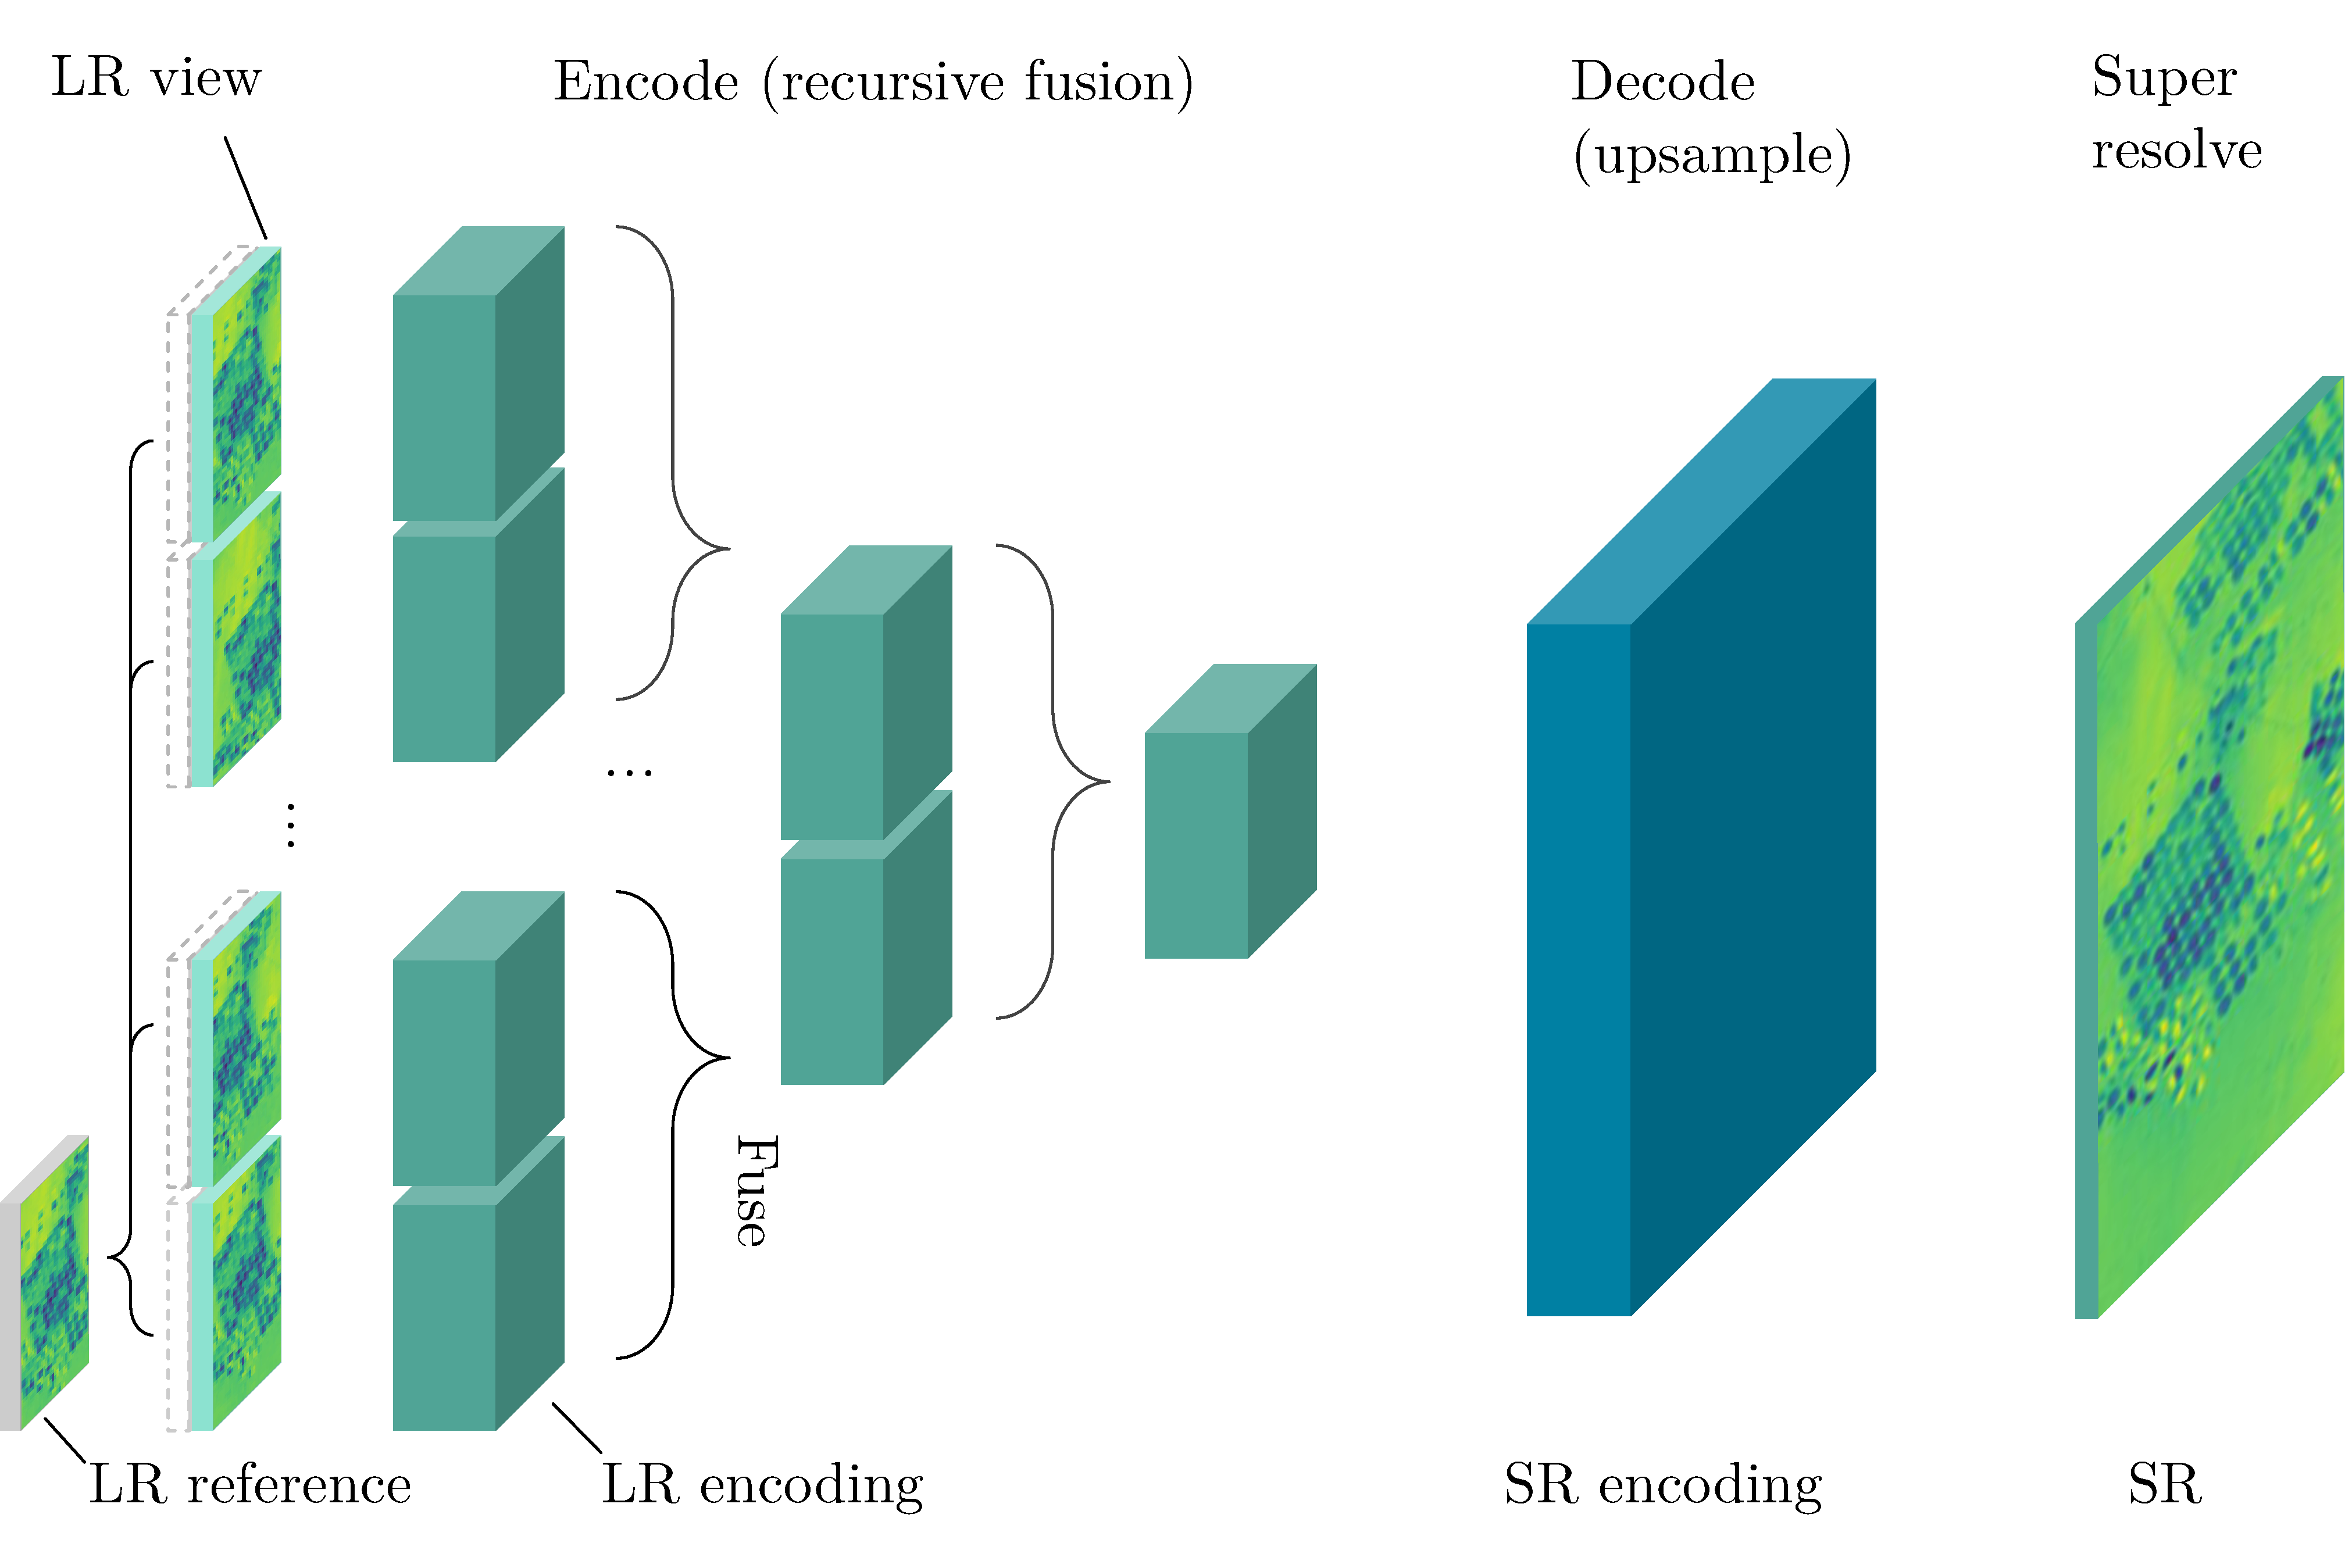
\includegraphics[width=\textwidth]{high_res_net_inference}
    \caption{Schematic of inference in \textit{HighRes--net} \cite{deudon-2020-highresnet}}
    \label{fig:highresnet-inference}
\end{figure}

The key element of \textit{HighRes--net} is achieving \textit{multi--frame super--resolution} by \textit{recursive fusion}.
Image generation is done by a neural network organized in an encoder--decoder scheme.
The input of the encoder is constructed from a series of low--resolution images.
If necessary, the input set is padded with zero--valued images to ensure that the number of low--resolution images is a power of 2, which is required by the network architecture.
For each input series, a \textit{reference image} is computed using median values of images.
Then the reference picture is paired with the input images.
Each low--resolution and reference pair is processed through an embedding function.
Embedding layers consists of a convolutional layer and two residual blocks with PReLu activations.
For input of length \textit{n}, output of the encoding consists of \textit{n} images, each convolved with the reference image.
In this scheme embedding learns to perform a process called \textit{implicit co--registration}, which is responsible for adjusting geometric differences between images in the input.
It is important to notice that the embedding block is a single instance shared between input pairs.

The next step in the \textit{HighRes--net} architecture is \textit{recursive--fusion}.
In this process output images are recursively fused together, pair by pair.
The fusion operation consists of two steps---co--registration of the input pair and the actual fusion.
The co--registration of fused images is similar to the co--registration of the input--reference pairs.
It is done by convolutional layer with PReLu activation and two residual layers.
Then the fusion itself is done, again by a combination of a convolutional layer and PReLu (this part doesn't include local residual layer).
The whole co--registration--fusion includes a residual connection.
Similarly to the embedding block, the fusion operator has a single instance that is shared for all steps of the recursion.

The last step of super--resolution process is to upscale the image by decoding the hidden state.
This is done with transposed convolutional layer with PReLu activation.
The transposition of the output of convolution makes the data grow in spatial dimensions, instead of the usual increase of depth when convolving.
The final image is constructed by applying convolution of size one, which doesn't change the size of the image.

\subsection{Registered loss calculation}
\label{sec:shiftnet}
As stated before, registration is an important part of \textit{HighRes--net} architecture.
It is especially crucial at the loss calculation step.
Without registration, the network would learn to output blurry images as a result of shift between predictions and targets.
Previous steps of \textit{HighRes--net} include an \textit{implicit co--registration}, where registration mechanisms learned by the network don't have to be necessarily based on shifts, but also other geometric distortions.
During evaluation it is desired to register image shifts explicitly, thus the \textit{registration--at--loss} differs from the registration performed during encoding and fusion.
At the final step, the sub--pixel registration is done by the \textit{ShiftNet--Lanczos} network.
\textit{ShiftNet} \cite{zhaoyi-2018-shiftnet} was introduced before \textit{HighRes--net}, in a separate research.
It was created with image inpainting via \textit{Deep Feature Rearrangement}.
Because this kind of filling in missing picture areas works by reusing and transferring existing data, it is suitable to be used as a registration mechanism.
It implements a modified \textit{U--Net} \cite{ronnenberger-2015-unet} architecture.
As mentioned in the introduction, U--Nets follow the encoder--decoder pattern with multiple residual connections.
Pairs of convolution and deconvolution layers in the contracting and expanding arms of a U--Net feature a residual connection.
The \textit{ShitNet} variant of \textit{U--Net} architecture contains an additional \textit{shift} operation for one of these residual connections.
More about \textit{ShiftNet} can be found in the publication.

\section{Other super--resolution architectures}
As mentioned, other super--resolution architectures are available, with RAMS \cite{salvetti-2020-rams} being the best performing one.
RAMS utilizes a novel technique called \textit{feature attention mechanism}, which enables the network to focus on high--frequency information that can be used to produce more detailed outputs.
This leads to overcoming main locality limitations of convolutional operations.
Mechanisms used in RAMS are specifically aimed at multi--image super--resolution of remote sensing data.
RAMS approach takes into account the nature of satellite imagery---relatively low spatial resolution and high depth and temporal resolution.
The attention mechanism works with three--dimensional convolutions to explore all possible directions.
This architecture puts emphasis on simultaneous data exploration and from spatial and temporal dimension resulting in the best quality of multi--image super--resolution.

\section{Resizing images with interpolation techniques}
Image resizing is a relevant topic in super--resolution, as a reference point and a tool for visualization.
It is useful as a visual baseline for super--resolution.
Traditional image resizing algorithms use interpolation to enable changing image dimensions; however, they do not create new details in the image.
A well--working super--resolution should recreate missing features when enhancing images.
Thus, it is expected that any super--resolution algorithm gives better results than image interpolation techniques.
In this work, image interpolation is used for comparisons during both the augmentation and super--resolution processes.

\subsubsection{Bicubic interpolation}
\textit{Bicubic interpolation} is one of the most prominent image interpolation modes.
Compared to other interpolation techniques it is regarded as the most advanced and time consuming of the commonly used solutions \cite{han-2013-interpolation} \cite{teoh-2008-inrepolation}.
This interpolation mode fills missing values by fitting third--degree polynomials between existing pixels.
The gradients of existing values are taken into account during the fitting process, so the interpolation splines' steepness matches the existing derivatives.
Bicubic interpolation is usually calculated in neighborhoods of four by four pixels.
Fitting polynomials to existing pixels may lead to \textit{overshooting} values.
This phenomenon often causes a slight increase in local contrast, which overall increases the \textit{acutance} (perceived sharpness) of an image.
Other image resizing modes operate on a simpler basis or consist in fitting simpler interpolation functions.
For this reason, bicubic is the most advanced and often best out of the common solutions.

\subsection{Other interpolation modes}
The bicubic interpolation has been chosen as a main reference point; however, there are other popular image resizing techniques that may be taken into account in comparisons.

The \textit{nearest neighbor interpolation} is the simplest out of widely used techniques.
In this approach the missing points are filled in with values of the closest existing pixels.
This technique often resolves in jagged edges and coarse details.

Another widely used approach is \textit{bilinear interpolation}.
Bilinear mode works similarly to bicubic one; however, it operates on simpler terms.
Instead of fitting polynomials it uses straightforward linear functions to find missing values.
Fot his reason, it cannot take into account image gradients and often results in less plausible outcome.
Furthermore, in contrast to the bicubic interpolation, bilinear usually operates in two by two neighborhoods.

\textit{Lanczos} is another interpolation method, with greater complexity and quality similar to bicubic.
In contrast to other techniques, it uses sinus function for interpolation.
Fitting is done using \textit{Lanczos filters} which may vary in function order and neighborhood size.

More details about various interpolation methods and function can be found in literature.




\chapter{Scope of the work}
\label{ch:scope}
This chapter provides a detailed plan of the proposed work and a rationale for chosen methods and technologies.
A subset of super-resolution and augmentation techniques is chosen to include in the course of the work.
Based on the selection, an experiment plan is laid out.
A brief description of utilized tools, technologies, and methodology to perform deep learning trainings is included.

\section{Selection of data types and augmentation techniques}
Various data types in the field of super-resolution and approaches to data augmentation were introduced in Chapters \ref{ch:introduction} and \ref{ch:analysis}.
A subset of possible techniques should be chosen to determine the scope of the experiments.

\subsection{Data types in super-resolution}
The introductory chapters provide a general overview of super-resolution, data augmentation mechanism, and types of satellite imagery.
To lay out a plan of experiments, a subset of selected techniques should be defined.
The previously described types of super-resolution training data are presented in the form of a graph in Figure \ref{fig:image-types}.
The graph features a distinction that has not been mentioned before---a difference between fully and semi-simulated multi-image datasets.
When multi-image training data generation is considered, one of two approaches can be taken.
If multiple high-resolution images of the same scene are available, then low-resolution training images can be created by shrinking each of the distinct photos.
This way of data generation can be denoted as \textit{semi-simulated}.
Otherwise, one can create many low-resolution images from a single high-resolution one.
This can be done by shifting the original image randomly multiple times and then, applying the shrinking transformation to each displaced copy.
This procedure is denoted as a \textit{(fully) simulated} data generation and is presented in the form of pseudocode as Algorithm \ref{alg:gen-simulated}.
\begin{figure}
	\centering
    \documentclass[tikz]{standalone}
\usepackage[utf8]{inputenc}

\usetikzlibrary{positioning}
\usetikzlibrary{shapes}
\usetikzlibrary{calc}

\begin{document}

\tikzstyle{cell} = [rectangle, rounded corners, minimum width=2cm, minimum height=1cm,text centered, draw=black]
\tikzset{arrow/.style={-stealth}}

\begin{tikzpicture}[ampersand replacement=\&]
	\node[cell, fill=blue!20] at (0,0) (D) {Data};
	
	\node[cell] at (0, 2) (FS) {Frequency spectrum};
	\node[cell] at (-2.5, 4) (MB) {Multi--band};
	\node[cell] at (2.5, 4) (SB) {Single--band};
	
	\node[cell] at (-4.5, -2) (MI) {Mulit--image};
	\node[cell] at (4.5, -2) (SI) {Single--image};
	
	\node[cell] at (-8, -4) (SIM) {Simulated};
	\node[cell] at (-4.5, -4) (SS) {Semi--simulated};
	\node[cell] at (-1, -4) (RLM) {Real--life};
	
	\node[cell] at (2.75, -4) (SIS) {Simulated};
	\node[cell] at (6.25, -4) (RLS) {Real--life};
	
	\node[cell] at (0, -6.5) (SM) {Simulation method};
	
	\node[cell] at (-2.5, -8.5) (T) {Traditional};
	\node[cell] at (-5, -10.5) (IM) {Interpolation modes};
	\node at (-2.5, -10.5) { $ \dots $ };
	
	
	\node[cell] at (2.5, -8.5) (DL) {Deep learning};
	\node[cell] at (1, -10.5) (NA) {Network architectures};
	\node at (3.75, -10.5) { $ \dots $ };

    \path[arrow]
    (D) edge (FS)
    (FS) edge (MB)
    (FS) edge (SB)
    (D) edge (MI)
    (D) edge (SI)
    (MI) edge (SIM)
    (MI) edge (SS)
    (MI) edge (RLM)
    (SI) edge (SIS)
    (SI) edge (RLS)
    (SIM) edge (SM)
    (SS) edge (SM)
    (SIS) edge (SM)
    (SM) edge (T)
    (SM) edge (DL)
    (T) edge (IM)
    (DL) edge (NA)
    ;
\end{tikzpicture}

\end{document}
    \caption{Graph of various training data generation techniques}
    \label{fig:image-types}
\end{figure}
\begin{algorithm}
\caption{Approach to generating fully simulated multi-image datasets}
\label{alg:gen-simulated}
\begin{algorithmic}
	\REQUIRE {$ n_{lr} $, $ ratio_{shrink} $}
	\STATE $ shift_{max} = ratio_{shrink} $
	\FORALL{$ hr_{img} $}
		\STATE $ hr_{cropped} = crop\_border(hr_{img}, shift_{max}) $
		\FOR{$ i = 0 $ \TO $ n_{lr} $}
			\STATE $ hr_{shift} = generate\_shift(shift_{max}) $
			\STATE $ hr_{translated} = translate(hr_{img}, hr_{shift}) $
			\STATE $ lr_{img} = downscale(hr_{translated}, ratio_{shrink}) $
			\STATE $ lr_{img}^{i} = crop\_border(lr_{img}) $
		\ENDFOR
		\STATE $ save\_scene(hr_{cropped}, lr_{img}^{i \dots n_{lr}}) $
	\ENDFOR
\end{algorithmic}
\end{algorithm}

A selection of approaches to be taken into account in this work has been made and marked with blue color in the graph in Figure \ref{fig:image-types}.
The choice is rather arbitrary and aims to cover the most common, yet uncomplicated variants of data generation.
Thus, it was decided to perform data augmentation for multi-image super-resolution on single-band pictures with simulated data using deep learning and resizing algorithms.

\subsection{Data augmentation techniques and approaches}
\subsubsection{Augmentation via deep learning}
Augmentation with deep learning techniques is the key point of this work.
In the subsequent chapters, three augmentation architectures with varying levels of complexity are introduced.
It should be kept in mind that this kind of augmentation requires a separate dataset to fit the augmentation networks prior to the export of the proper super-resolution training data.

\subsubsection{Augmentation via interpolation algorithms}
In the process of the work, the deep learning-based augmentation methods are to be compared with traditional resizing algorithms which are based on interpolation techniques.
The \textit{bicubic interpolation} was chosen as a reference point.
Furthermore, the images created with bicubic interpolation were subject to several transformations to enhance their quality.
The brightness, contrast, and noise of the interpolated images were adjusted using normal distributions with parameters:
\begin{description}
	\item[Gaussian noise] with 0.0 mean and standard deviation of 30 was applied to each image.
	\item[Contrast] was adjusted by multiplying each image by random scalar value from gaussian distribution with 1.0 mean and standard deviation of 0.2.
	\item[Brightness] was adjusted by adding a random scalar value from gaussian distribution with 0.0 mean and standard deviation of 200 to each image.
	\item[Gaussian blur] with a standard deviation of 0.5 was applied to each of these low-resolution images.
\end{description}
These were applied to Sentinel-2 images with values in 14-bit (maximum value is 16384) range.
These transformations applied to the dataset created by bicubic interpolation were chosen outside of the scope of this work.

\subsubsection{Translations between low-resolution images in multi-image super-resolution data}
As stated before, in this work multi-image super-resolution is taken into account.
When generating images with both interpolation and deep learning techniques, the same approach to creating translations between low-resolution images was taken.
These were created using uniform distribution between $-0.95$ and $0.95$ in the high-resolution domain.
The translations were applied in the vertical and horizontal directions.

\section{Plan of experiments}
After choosing a subset of augmentation techniques to examine, an experiment plan should be laid out.

\subsection{Required data}
The broad aim of the work is to train augmentation neural networks on small real-world datasets and then use the trained models to export a larger, synthetic dataset which should be used to fit a super-resolution algorithm.
A number of datasets are required to perform this task.
To clarify the demands for specific datasets can be listed as:
\begin{enumerate}
	\item A dataset containing high and low-resolution images for training an augmentation network.
	\item A dataset containing high and low-resolution images for testing the augmentation network.
	\item Dataset that should be augmented with the network.
	      This set does not need to contain high and low-resolution pairs.
	      The low-resolution images for existing high-resolution ones should be generated by the augmentation network.
	      Results of the augmentation will be used to train the super-resolution network.
	 \item Dataset of high and low-resolution images for testing the super-resolution network.
\end{enumerate}

\subsubsection{Proba-V as an augmentation training dataset}
\label{sec:probav}
The \textit{Proba-V} dataset \cite{esa-proba} can be used to fill the first two requirements.
It contains images taken during the \textit{Proba-Vegetation} satellite mission launched by the \textit{European Space Agency} in 2013.
The dataset contains imagery taken in multiple spectral bands.
Two subsets are regarded in this work---the \textit{\gls{red}} band (610--690 \si{\nano\meter} wavelength) and the \textit{\gls{nir}} band (777--893 \si{\nano\meter} wavelength).
Proba-V contains multiple real-life low-resolution images per one high-resolution image.
Images of the same scene were taken in different moments, thus they vary slightly in framing and atmospheric conditions.
Unprocessed Proba-V high-resolution images are 384 by 384 pixels, low-resolution photos are 128 by 128 pixels.
As mentioned in Chapter \ref{ch:analysis} high-resolution images have \gls{gsd} of $ 1/3 \times 1/3 $ kilometer per pixel and the low-resolution ones feature \gls{gsd} of $ 1 \times 1 $ kilometer per pixel \cite{direckx-2013-proba}.
A selected pair of high and low-resolution samples from the Proba-V dataset is shown in Figure \ref{fig:proba-sample}.
\begin{figure}[htb!]
    \begin{subfigure}{0.45\textwidth}
        \centering
        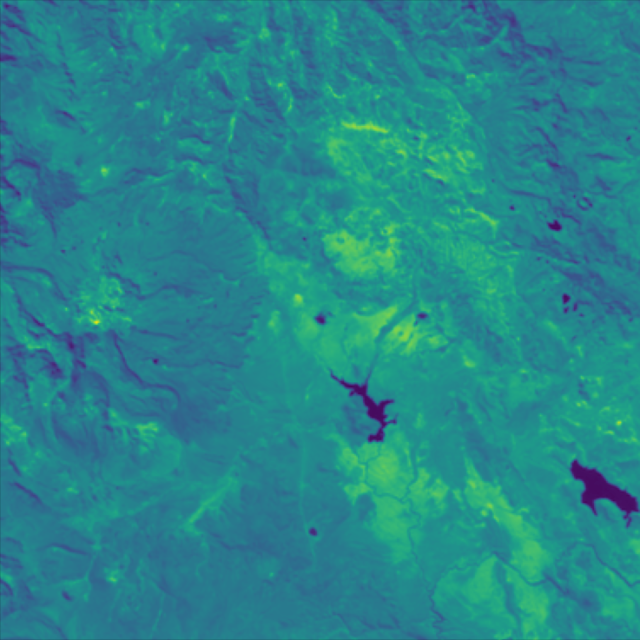
\includegraphics[width=\textwidth]{sample_nir_hr}
        \caption{High-resolution image}
    \end{subfigure}
    \hfill
    \begin{subfigure}{0.45\textwidth}
        \centering
        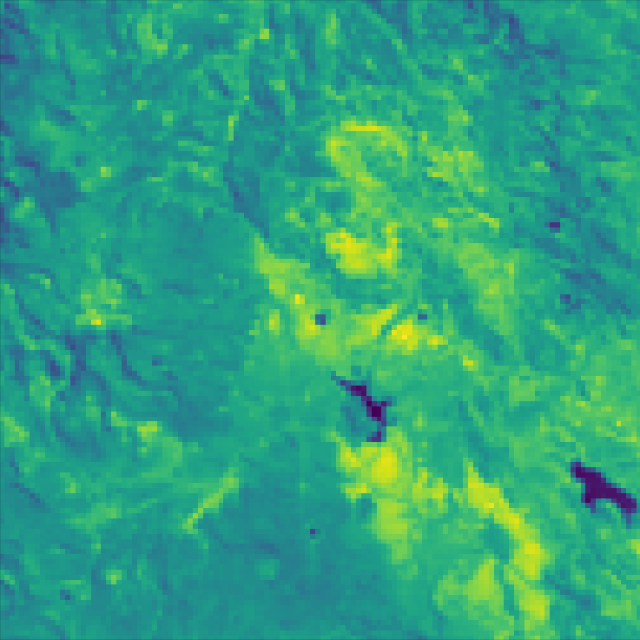
\includegraphics[width=\textwidth]{sample_nir_lr}
        \caption{Low-resolution image}
    \end{subfigure}
    \caption{Sample image pair from \textit{Proba-V \gls{nir} train dataset}}
    \label{fig:proba-sample}
\end{figure}
Furthermore, Proba-V features a set of binary masks for low-resolution images.
These masks indicate areas of photos that may not be suitable for processing, such as clouds or blank spaces.
An example of a Proba-V image with a binary mask designating clouds is shown in Figure \ref{fig:proba_sample_mask}.
\begin{figure}[htb!]
    \begin{subfigure}{0.45\textwidth}
        \centering
        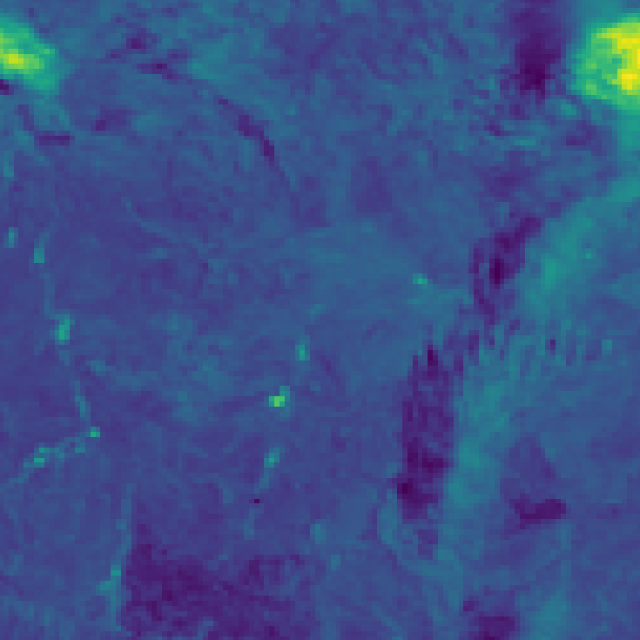
\includegraphics[width=\textwidth]{proba_sample_clouds}
        \caption{Sample Proba-V image with invalid areas that contain clouds}
    \end{subfigure}
    \hfill
    \begin{subfigure}{0.45\textwidth}
        \centering
        
\includegraphics[width=\textwidth]{proba_sample_mask}
        \caption{Binary mask for a sample Proba-V image with invalid area}
    \end{subfigure}
    \caption{Proba-V sample with invalid area and its binary mask}
    \label{fig:proba_sample_mask}
\end{figure}
Proba-V pictures are saved as 16-bit images; however, only 14 bits are used to store pixel values.

\subsubsection{Sentinel-2 as a super-resolution training dataset}
The super-resolution training part of the data demands can be met by utilizing \textit{Sentinel-2} dataset \cite{esa-sentinel}.
Contrary to Proba-V, it does not feature high and low-resolution scenes, for this reason, it suits the role of the dataset to undergo the data generation process.
Sentinel-2 is a part of the European Earth Observation Program that has lasted since 2015.
It gathers data from two twin satellites that acquire optical imagery at high spatial resolution from 10 to 60 meters.
Sentinel-2 images are multi-spectral and feature a total of 13 bands with \gls{gsd} values of $ 10 \times 10 $, $ 20 \times 20 $ and $ 60 \times 60 $ meters per pixel \cite{tas-sentinel}.
Since it was decided not to include multi-spectral super-resolution only band eight is to be used.
This band features spectrum close to infrared (835.1 nm central wavelength, 145 nm bandwidth for satellite Sentinel-2~A and 833 nm central wavelength, 133 nm bandwidth for satellite Sentinel-2~B) with \gls{gsd} of $ 10 \times 10 $ meters per pixel).
A sample image from the Sentinel-2 dataset is shown in Figure \ref{fig:sentinel_sample}.
\begin{figure}
	\centering
    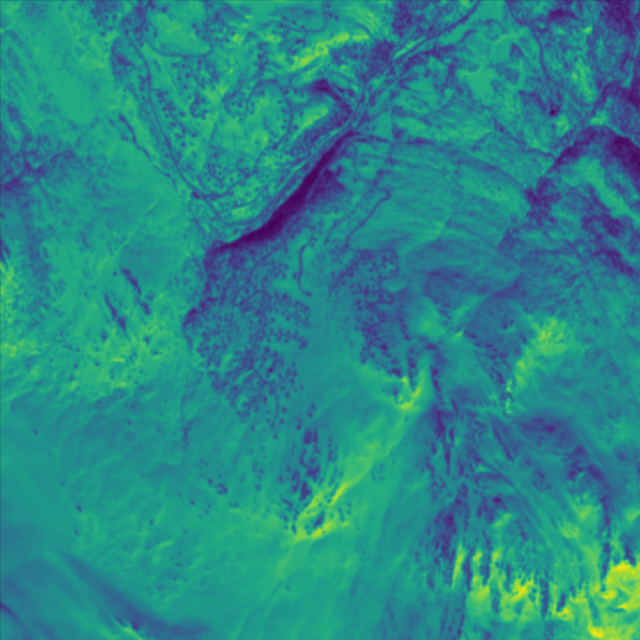
\includegraphics{sentinel_sample}
    \caption{Sample image from \textit{Sentinel-2 dataset} (eight band)}
    \label{fig:sentinel_sample}
\end{figure}
As with Proba-V, Sentinel-2 is saved using 16-bit image format; however, only 14 bits store useful pixel values.

\subsubsection{Dataset for super-resolution evaluation}
Additional datasets are needed to evaluate the final results.
The goal of the tests is to measure super-resolution generalization capabilities and data selection impact on the metrics.
This can be done in four ways with different data:
\begin{itemize}
	\item Each augmented Sentinel-2 dataset should contain a test subset. Each super-resolution network can be evaluated on a test set generated in the same way as that used for the training.
	\item Test subsets generated in different forms can be used in a cross-type evaluation scheme. In this work, the augmented datasets are created in a variety of ways. The network trained on one version of an augmented dataset can be tested on a dataset created using a different method. For example, a super-resolution network trained using the data created with bicubic interpolation can be tested on the data generated by a neural network (and the other way). These cross-type tests can be used to examine generalization capabilities.
	\item Separate real-world Sentinel-2 images can be used for tests. Sentinel-2 does not include high and low-resolution pairs, so numeric tests are not possible. However, it is still viable to perform a visual test, for example, in search of artifacts.
	\item The Proba-V test subset used to evaluate the augmentation process can be used to measure super-resolution performance. Since the initial tests are not a part of any decision process, there is no information leak and the Proba-V subset can be used twice.
\end{itemize}

\subsection{Experiment flow}
Given the selection of data augmentation methods and available data an experiment flow can be laid out in the form of a graph in Figure \ref{fig:experiment-flow}.
The experiment flow presented in the graph is as folows:
\begin{enumerate}
	\item Use existing real-life Proba-V dataset to train augmentation networks.
	\item Take the existing Sentinel-2 dataset (which features single-resolution images). Use the augmentation networks to create Sentinel-2 datasets with high and low-resolution image pairs. These datasets are designated as \textit{degraded} in the graph.
	\item Use the single-resolution Sentinel-2 and bicubic interpolation to create another version of the Sentinel-2 dataset with high and low-resolution pairs.
	\item The generated Sentinel-2 datasets should contain subsets for training and testing super-resolution networks.
	\item Use all the generated datasets to train the HighRes-net super-resolution network.
	\item Evaluate the super-resolution networks using various datasets:
	\begin{enumerate}
		\item Evaluate networks on the test subsets associated with the training sets. Test each network on the data created in the same way as its training set.
		\item Use the generated test subsets to perform the cross-type evaluation. Test the networks on the image sets created differently from the training data.
		\item Use the Proba-V test subset to evaluate results of training HighRes-net on different datasets.
		\item Use the separate real-life single-image Sentinel-2 data to perform visual checks.
	\end{enumerate} 
\end{enumerate}
\begin{figure}
	\centering
	\documentclass[tikz]{standalone}
\usepackage[utf8]{inputenc}

\usetikzlibrary{positioning}
\usetikzlibrary{shapes}
\usetikzlibrary{calc}

\begin{document}

\tikzstyle{cell} = [rectangle, rounded corners, minimum width=3cm, minimum height=1cm,text centered, draw=black, fill=white, align=center]
\tikzset{arrow/.style={-stealth}}

\begin{tikzpicture}[ampersand replacement=\&]
	\node[cell, fill=blue!20, align=center] at (1,0) (PVTS) {Proba-V train set \\(High and low-resolution pairs)};
	\node[cell] at (-5,0) (ANA) {Augmentation\\network achitecture};
	
	\node[cell, fill=blue!20] at (0.5,-2) (S2TS) {Sentinel-2 set\\(single-resolution)};
	\node[cell] at (-5,-2) (TAN) {Trained augmentation\\network};
	
	\node[cell] at (6,-2) (BIC) {Downsizing\\with bicubic interpolation};
	
	\node[cell, fill=blue!20] at (-1.5,-4.5) (SDTR) {Sentinel-2 degraded\\train set};
	\node[cell, align=center, fill=blue!20] at (-4.5,-5) (SDTS) {Sentinel-2 degraded\\test set};

\node[cell, fill=blue!20] at (6.5,-4.5) (SBTR) {Sentinel-2 bicubic\\train set};
	\node[cell, fill=blue!20] at (3.5,-5) (SBTS) {Sentinel-2 bicubic\\test set};
	
	\node[cell] at (1,-8.5) (HRNA) {HighRes-net\\architecture};
	
	\node[cell] at (6,-8.5) (HRNTB) {HighRes-net\\trained on bicubic};
	\node[cell] at (-4,-8.5) (HRNTD) {HighRes-net\\trained on degraded};
	
	\node[cell, fill=blue!20] at (-4,-11) (SR) {Sentinel-2 real test set\\(single-resolution)};
	\node[cell, fill=blue!20] at (6,-11) (PT) {Proba-V test\\(High and low-resolution pairs)};

    \path[arrow]
    (PVTS) edge (ANA)
    (ANA) edge (TAN)
    (S2TS) edge (TAN)
    (S2TS) edge (BIC)
    (BIC) edge (SBTR)
    (BIC) edge (SBTS)
    (TAN) edge (SDTR)
    (TAN) edge (SDTS)
    (SDTR) edge[bend right] (HRNA.north west)
    (SBTR) edge[bend left] (HRNA.north east)
    (HRNTB) edge[dashed] (SDTS) 
    (HRNTD) edge[dashed] (SDTS)
    (HRNTB) edge[dashed] (SBTS)
    (HRNTD) edge[dashed] (SBTS)
    (HRNA) edge (HRNTB)
    (HRNA) edge (HRNTD)
    (HRNTD) edge[dashed] (SR)
    (HRNTD) edge[dashed] (PT)
    (HRNTB) edge[dashed] (SR)
    (HRNTB) edge[dashed] (PT)
    ;
\end{tikzpicture}

\end{document}
	\caption{Graph of the experiment flow (solid lines indicate trainings, dashed arrows designate evaluations, blue stands for datasets, white is for models and algorithms)}
	\label{fig:experiment-flow}
\end{figure}

\section{Selection of tools and technologies}
The implementation of the experiment plan requires a selection of programming tools.
Subsequent sections provide a rationale for choosing a set of necessary technologies and libraries to accomplish the project's goals.

\subsection{Language and libraries}
\textit{Python}, which is an industry-standard for neural network research and scientific computing has been chosen as the main language for the implementation.
It combines the ease of prototyping new code with the efficient use of existing libraries written in more performant languages.
Python version 3.8 was chosen for the project as a reasonably recent, yet mature and field-tested version.

The main part of the work which consists in writing neural network architectures and training them was written using the \textit{Tensorflow} library.
Tensorflow has been a leading deep learning library in recent years and is widely used in the industry and academia.
Version 2.5 of the library was chosen for the project.
From the second version, Tensorflow includes \textit{Keras} neural network prototyping interface natively as default and recommended way for model building.
This work utilizes the Keras API as well as some underlying Tensorflow functions for fine-tuning and expanding models.
Tensorflow supports \gls{gpu} acceleration via \textit{NVIDIA CUDA} libraries, which is crucial for conducting efficient trainings.

The image manipulation tasks are performed using the \textit{SciKit-image} library which offers a variety of utilities, transformations, and analysis tools.
\textit{Matplotlib}, another wide-spread Python library was used to create plots and heatmaps in the work.
Alongside SciKit-image, \textit{Pillow} was used for some image-related operations (mainly for resizing images with specific interpolation modes).

\textit{NumPy}, the most popular numerical calculations library was chosen as a tool for matrix manipulation and mathematical operations.
Arrays created with NumPy are stored in a contiguous memory layout, which enables the utilization of performance optimizations such as vectorized operations. 
NumPy ubiquity in the world of scientific computing with Python proves to be very convenient.
It is compatible with other popular libraries; it is interoperable with parts of Keras API, Scikit-image stores images as NumPy arrays, Matplotlib can plot data from NumPy arrays out-of-the-box.
NumPy arrays' performance comes from their static nature, as their size is predetermined.
This constrain is a prerequisite to the contiguous memory layout of the arrays, which enables the utilization of fast mathematical operations.
However, this comes at a cost of flexibility; resizing the NumPy arrays is costly and often requires substantial memory reallocations.

The set of required libraries with proper versions can be installed using \textit{requirements.txt} files.
It is best to use it inside a Python \textit{virtualenv}, running the command: \mintinline[breaklines]{shell}{pip install -r requirements.txt}.

To ensure code quality and avoid mistakes, a \textit{continuous integration} system was used.
Continuous integration is based on automatic code building on the server with the help of version control systems.
Every time a new commit is pushed to the upstream, a set of checks is run remotely.
The integration system reports any errors and prevents the integration of invalid code into the main system.
The built-in GitHub continuous integration and delivery system, called \textit{GitHub Actions} was used in the project.
Integration checks are performed inside a Ubuntu Docker image and consist of various \textit{flake8} linter analytics.

\subsection{Data and experiment management}
\label{sec:exp-management}
The codebase in the work was managed with the \textit{Git} version control system.
Git is the most popular tool for tracking changes in code and text files.
However, it was not created with media and datasets in mind.
Git may work very slowly with large data and popular Git server providers such as \textit{GitHub} offer limited storage for repositories.
For this reason, \textit{\gls{dvc}}---a supplementary tool was used.
\gls{dvc} consists of two main components: data versioning and experiment tracking.
The data versioning part is similar to systems like \textit{Git LFS}; it stores metadata inside the Git repository and the actual data in other storage (e.g. Google Drive).
Information about the proper data is stored in the form of \textit{MD5} hashes in the metadata files.
The metadata versioned with Git can be used to download proper data from the external cloud storage.
\gls{dvc} is analogous to Git in operation, it uses a command-line interface with a similar structure.
To download the data in the project one should run the command \mintinline{shell}{dvc pull}.
Since the metadata is versioned with Git, when going back in the commit history one should run \mintinline{shell}{dvc checkout} after \mintinline{shell}{git checkout} to conceal data versions.

The experiment tracking part of \gls{dvc} ensures reproducibility and results caching.
The layout of experiments is stored in the \textit{dvc.yaml} file where each stage of experiment is described with its input dependencies and outputs.
The results of each stage can be cached and rebuilt automatically depending on changes in the dependencies.
The experiments in this work usually depend on data and files with model architecture.
Training models can be parametrized using a configuration file, here named \textit{params.yaml}.
Parameters of models and training can be changed by editing this file.
Another convenience of \gls{dvc} is that the outputs are automatically rebuilt on changes in the parameters.
Trained models are cached and bound with code and parameters used for training.
Like the data versioning system, models and artifacts are also tracked with metadata and git.
When going back with history, \mintinline{shell}{dvc checkout} will also conceal artifacts and data.
The stage of the experiment pipeline is stored in the \textit{dvc.lock} file that also contains metadata.
The command \mintinline{shell}{dvc repro} is used to reproduce experiments; however, scripts in the project can also be run independently of \gls{dvc} (more details about reproducing experiments can be found in Appendix \ref{ch:appendix-technical}).

\section{Project strucutre}
Files in the project have the following structure and function:
\begin{description}
	\item[.github/workflows/build.yml] continuous integration system configuration.
	\item[cnn\_res\_degrader] main part of the source code, contains the augmentation models, training, and testing scripts.
	\item[dataset\_augmentation] source code for exporting augmented Sentinel-2 datasets.
	\item[data] super-resolution datasets and artifacts controlled by \gls{dvc}.
	\item[dvc.lock] metadata to track experiment progress in the current commit.
	\item[dvc.yaml] DVC experiment description.
	\item[params.yaml] models and experiment configuration.
	\item[requirements.txt] libraries requirements.
\end{description}
Some configuration files and minor parts of the project were omitted in this description.


\chapter{Data augmentation with usage of deep learning}
\label{ch:augmentation}
\section{Proba--V preprocessing}
As stated before, it was decided to use Proba-V as the augmentation training dataset.
As a preprocessing step, before training the high and low--resolution images should be aligned.
Some architectures, like the \textit{HighRes--net} feature deep learning based built--in mechanisms for image registration.
However, for training a simple image--downscaling augmentation network, a more traditional approach to image alignement can be implemented.
The preparation of dataset requires to turn the single high--resolution and multiple low--resolution imageset into high and low--res pairs.
This can be done by multiplying high--resolution images and aligning each copy with the corresponding low--resolution one.

Among the image registration algorithms presented in Section \ref{sec:registration}, phase-correlation was chosen for aligning image pairs in the Proba dataset.
This method is suitable for the preprocessing task and is implemented as a part of popular image processing libraries.
Since pictures to be aligned in Proba are of different resolution, they should be resized to a common shape before registration.
It was decided to perform registration in the high--resolution image domain.
Shifting images will create blank columns and rows on their borders, which were removed by cropping the images.
It is known that low--resolution images in Proba have sub--pixel dislocation, for this reason they should be cropped with one pixel border.
High--resolution images are three times larger, consequently, a margin of three pixels should be removed from them.
After this step of preprocessing high--res images are 378 by 378 pixels and low--resolution photos are 126 by 126 pixels.
It is valuable to visualize the effects of the registration process to ensure its correctness.
Because Proba images have single depth dimension, they can be visualized as different color channels.
This technique is utilized in the figure \ref{fig:proba-registration}, where red and blue channels contain two pictures that are to be registered.
If the pictures are aligned perfectly, the image should be yellow because red and blue channels overlay perfectly.
The more unaligned the pictures are the more red and blue is visible in the picture, which is most visible at distinct edges.
The visualization proves that the phase--correlation based registration is suitable for the Proba--V dataset---after registration the picture becomes more yellow and the unaligned edges are less visible.
\begin{figure}
    \begin{subfigure}{0.45\textwidth}
        \centering
        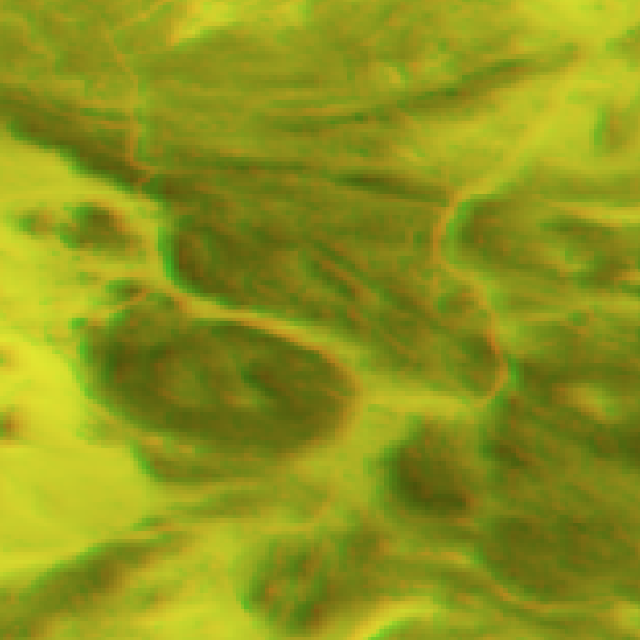
\includegraphics[width=\textwidth]{proba_unregistered}
        \caption{Proba--V images overlay before registration}
    \end{subfigure}
    \hfill
    \begin{subfigure}{0.45\textwidth}
        \centering
        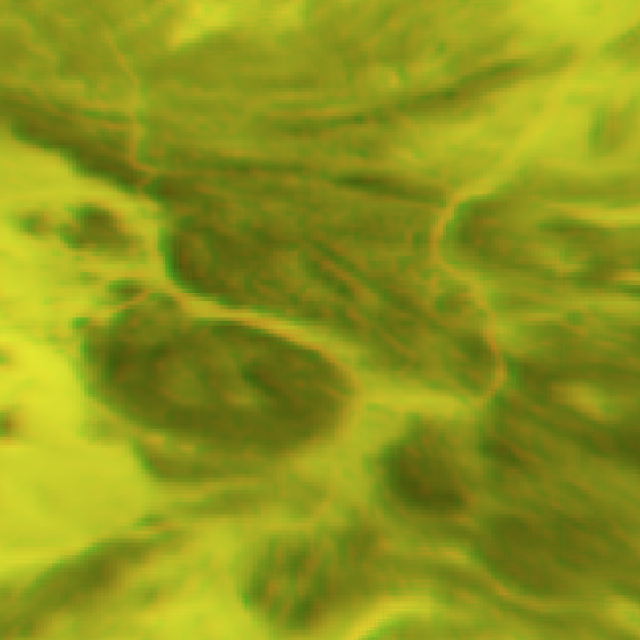
\includegraphics[width=\textwidth]{proba_registered}
        \caption{Proba--V images overlay after registration}
    \end{subfigure}
    \caption{Sample image pair from \textit{Proba--V NIR train dataset}}
    \label{fig:proba-registration}
\end{figure}

Photos in the Proba--V dataset are saved as sixteen-bit images; however, only fourteen--bit values are utilized.
It should be noted, to scale the images properly.
Using Proba--V dataset with real--life high and low--resolution images poses an additional challange.
As stated, the images contained in the dataset are taken at different moments, thus they differ in exposure and contrast.
Images in high and low--res pairs differ in brightness, both at the level of local details and global average values.
Distributions of image exposure in the dataset are presented in the figures \ref{fig:exposure-dist-red} and \ref{fig:exposure-dist-red} for RED and NIR subsets.
\begin{figure}
        \centering
         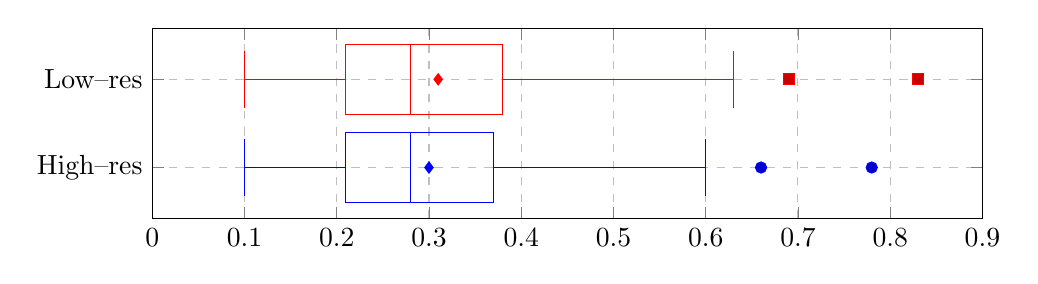
\begin{tikzpicture}
		 \begin{axis}[width=\textwidth, height=4cm, grid=major, grid style={dashed}, xmin=0, xmax=0.9, ytick={1, 2}, yticklabels={High--res, Low--res}]
		      \addplot+ [boxplot prepared={draw position=1,
		      							   average=0.30,
		                                   median=0.28,
		                                   lower whisker=0.1,
		                                   upper whisker=0.60,
		                                   upper quartile=0.37, 
		                                   lower quartile=0.21}] 
		                                   coordinates {(1,0.78)(1,0.66)};
		       \addplot+ [boxplot prepared={draw position=2,
		      							   average=0.31,
		                                   median=0.28,
		                                   lower whisker=0.10,
		                                   upper whisker=0.63,
		                                   upper quartile=0.38, 
		                                   lower quartile=0.21}] 
		                                   coordinates {(2,0.83)(2,0.69)};
		  \end{axis}
		  \end{tikzpicture}
    \caption{Exposure distributions in the RED Proba--V dataset}
    \label{fig:exposure-dist-red}
\end{figure}
\begin{figure}
        \centering
                 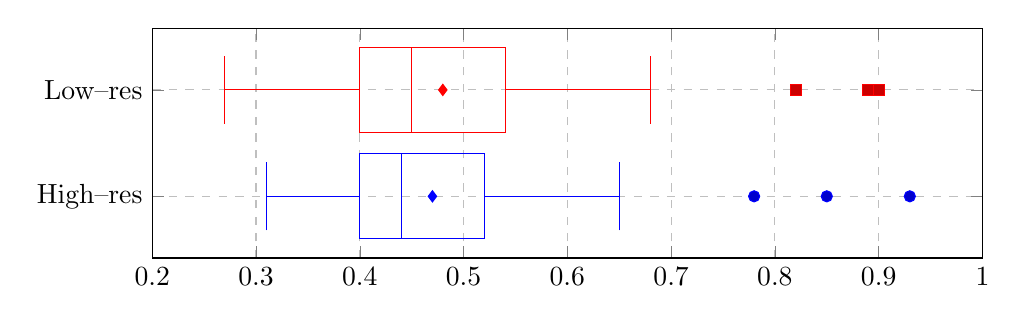
\begin{tikzpicture}
		 \begin{axis}[width=\textwidth, height=4.5cm, grid=major, grid style={dashed}, xmin=0.2, xmax=1, ytick={1, 2}, yticklabels={High--res, Low--res}]
		      \addplot+ [boxplot prepared={draw position=1,
		      							   average=0.47,
		                                   median=0.44,
		                                   lower whisker=0.31,
		                                   upper whisker=0.65,
		                                   upper quartile=0.52, 
		                                   lower quartile=0.40}] 
		                                   coordinates {(1,0.93)(1,0.85)(1,0.78)};
		       \addplot+ [boxplot prepared={draw position=2,
		      							   average=0.48,
		                                   median=0.45,
		                                   lower whisker=0.27,
		                                   upper whisker=0.68,
		                                   upper quartile=0.54, 
		                                   lower quartile=0.40}]
		                                   coordinates {(2,0.90)(2,0.89)(2,0.82)};
		  \end{axis}
		  \end{tikzpicture}
    \caption{Exposure distributions in the RED Proba--V dataset}
    \label{fig:exposure-dist-red}
\end{figure}


Having a dataset with high and low--resolution images of different brightness and contrast can be an obstacle for learning a neural network.
For this reason, \textit{histogram equalization} was applied to the learning data.
This technique enhances image contrast and evens the histogram of pixel values.
After equalization, the cumulative distribution of brightness is close to linear.

As noted previously, Proba--V includes binary masks denoting areas of images that are suitable for training.
Some images include noticeable large areas of unusable pixels.
For this reason, nine images with the least the percentage of invalid pixels were chosen per scene as training data.
This excludes incorrect data from the training set.  

\section{Augmentation network architectures}
The augmentation network is to perform a rather simple task of reducing the size of input pictures.
Three architectures that perform this task have been created, they are presented with an increasing complexity.

\subsection{Simple fully--convolutional network}
The most simplistic approach to shrinking images with deep learning is to build a basic, fully convolutional network.
The most simplistic implementation of this idea uses three convolutional layers with kernels of size three by three.
The midmost convolution slides the filter window with a stride of three to decrease the size of input by three times.
The last convolutional layer features one filter to reduce the output depth to a single channel.
\textit{ReLU} activation function was used for each applicable layer.
A precise description of the architecture is presented in the table \ref{tab:simple-conv-arch}.
\begin{table}
    \centering
    \caption{Simple fully--convolutional network architecture for data augmentation}
    \label{tab:simple-conv-arch}
    \begin{tabular}{ccc}
        \toprule
        Layer type & Output Shape & Number of parameters \\
        \midrule
        $ Input $      & 378, 378, 1  & 0                    \\
        $ Conv2D(filters=64, stride=1) $ & 378, 378, 64 & 640 \\
        $ ReLu $ & 378, 378, 64 & 0 \\
        $ Conv2D(filters=64, stride=3) $ & 126, 126, 64 & 36928 \\
        $ ReLU $ & 126, 126, 64 & 0 \\
        $ Conv2D(filters=1, stride=1) $ & 126, 126, 1 & 577 \\
        $ Sigmoid $ & 166, 126, 1 & 0 \\
        \bottomrule
    \end{tabular}
\end{table}

\subsection{Fully--convolutional encoder--decoder network}
The more complex architecture that can be applied is based on the previously mentioned encoder--decoder network scheme.
It is one of the most popular image--to--image neural network architectures.
The encoder shrinks the image by a factor of six instead of three.
Then the image is upscaled two times.
In result, the output image is overall three times smaller; however, it has been processed by more convolutional layers than in the simple convolutional network.

There are various ways to upscale the image during the decoding process.
The main ones are traditional upscaling and a \textit{transposed convolution} (sometimes called \textit{deconvolution}).
The later performs a convolution and then transposes the output, which makes the spatial dimension grow in size.
However, the transposed convolution layers can produce visible checkerboard artifacts on the image \cite{odena-2016-deconvolution}.
For this reason, the simpler layer architecture based on upscaling was chosen.
Like the simple architecture, the encoder--decoder features a convolution with a single filter at the end.
The detailed description of the network is shown in the table \ref{tab:autoencoder-arch}.
\begin{table}
    \centering
    \caption{Encoder--decoder network architecture for data augmentation}
    \label{tab:autoencoder-arch}
    \begin{tabular}{ccc}
        \toprule
        Layer type & Output Shape & Number of parameters \\
        \midrule
        $ Input $      & 378, 378, 1  & 0                    \\
        $ Conv2D(filters=64, stride=1) $ & 378, 378, 64 & 640 \\
        $ ReLU $ & 378, 378, 64 & 0 \\
        $ Conv2D(filters=64, stride=3) $ & 126, 126, 64 & 36928 \\
        $ ReLU $ & 378, 378, 64 & 0 \\
        $ Conv2D(filters=64, stride=2) $ & 126, 126, 64 & 36928 \\
        $ ReLU $ & 378, 378, 64 & 0 \\
        $ UpSampling2D(stride=2) $ & 126, 126, 64 & 0 \\
        $ Conv2D(filters=1, stride=1) $ & 126, 126, 1 & 577 \\
        $ Sigmoid $ & 166, 126, 1 & 0 \\
        \bottomrule
    \end{tabular}
\end{table}

\subsection{Generative adversarial network}
In recent years, a new approach to training generative neural networks has emerged.
The traditional supervised learning described in the previous sections consists in providing the network with an input and comparing the generated output with a ground truth to compute loss.
The \textsc{gan}---\textit{generative adversarial network} approach requires creating two networks, a \textit{generator} and \textit{discriminator} \cite{goodfellow-2014-gans}.
The former is tasked with generating data, while the latter learns to differentiate images created by the generator from real ones.
In the \textsc{gan} scheme the discriminator learns like a traditional binary classifier---it is provided with real and generated images, which are labeled accordingly.
Then discriminator loss is computed using standard classification metrics like \textit{binary cross--entropy}.
However, the generator learns in a more unique way; it creates an output image that is fed into a discriminator.
The generator loss is calculated depending on how well it produces data that may be classified as \textit{real} by a discriminator.
If the generated image is recognized as a \textit{fake} one, it receives a big penalty in the form of a large loss.

\textsc{Gan}s can have many variations, the most common variant utilizes unsupervised or semi--supervised data generation.
A great advantage of this kind of network is the ability to create images without direct input.
Usually a \textsc{gan} generator creates output from random values.
These values are randomly initiated inside proper \textit{latent space}.
However, adversarial networks can also work in fully--supervised way.
In this work a \textsc{gan} is proposed that transforms high--resolution images to low--resolution, with loss calculated in regard to the discriminator's judgements.
Such networks are often called picture--to--picture \textsc{gan}s.
An algorithm for training such a network is provided in the pseudocode listing \ref{alg:gan-training}.
One further optimization can be applied to \textsc{gan}---usually better results are achieved if small noise is applied to the labels.
\begin{algorithm}
\caption{\textsc{Gan} training flow}
\label{alg:gan-training}
\begin{algorithmic}
	\REQUIRE{$ x $, $ y_{gt} $}
	\STATE $ y_{fake} = generator(x) $
	\STATE $ y_{pred} = discriminator(cat(y_{fake}, y_{gt})) $
	\STATE $ loss_d = lossfn_d(y_{pred}, cat(\mathds{O}, \mathds{1})) $
	\STATE $ optimze_d(loss_d) $
	\STATE $ freeze\_learning(discriminator) $
	\STATE $ y_{pred} = discriminator(generator(x)) $
	\STATE $ loss_g = lossfn_g(y_{pred}, \mathds{1}) $
	\COMMENT{Notice the misleading labels matrix}
	\STATE $ optimize_g(loss_g) $
\end{algorithmic}
\end{algorithm}
The fitting process of a \textsc{gan} network can also be visualized in the form of a graph, as presented in the figure \ref{fig:gan-training}.
\begin{figure}
    \centering
    \documentclass[tikz]{standalone}
\usepackage[utf8]{inputenc}

\usetikzlibrary{positioning}
\usetikzlibrary{shapes}
\usetikzlibrary{calc}

\begin{document}
	
\tikzset{arrow/.style={-stealth}}

\begin{tikzpicture}[ampersand replacement=\&]
   	\node[text width=0.25cm] at (-2.5,0) (X) {$ \mathbf x $};		 
    \node[rectangle, rounded corners, draw, fill=blue!20, minimum height=1cm] at (0,0) (G) {\textsc{Generator}};	
    \node[rectangle, rounded corners, draw, minimum height=1cm] at (3,0) (S1) {\textsc{Sample}};
    
    \node[text width=0.5cm] at (0.75,3) (Y) {$ \mathbf y_{gt} $};		 
    \node[rectangle, rounded corners, draw, minimum height=1cm] at (3,3) (S2) {\textsc{Sample}};
    
    \node[rectangle, rounded corners, draw, fill=blue!20, minimum height=1cm] at (6,1.5) (D) {\textsc{Discriminator}};
    
    \node[text width=2cm] at (10,1.5) (O) {\textsc{Real/Fake Prediction}};
     
    \path[arrow] (X) edge (G)
    (G) edge (S1)
    (S1) edge (D.south west)
    (Y) edge (S2)
    (S2) edge (D.north west)  
    (D) edge (O)
    ;
\end{tikzpicture}

\end{document}
    \caption{Schematic of \textsc{gan} network inner--workings}
    \label{fig:gan-training}
\end{figure}
The final Tensorflow 2 implementation of the custom training loop step is shown in the listing \ref{lst:train_step_gan}.
\begin{listing}
\begin{minted}{python}
def train_step(self, data):
        x, y, y_mask = data
        batch_size = tf.shape(x)[0]

        y_fake = self.generator(x)

        # Discriminator training
        discriminator_input = tf.concat([y_fake, y], axis=0)
        fake_labels = tf.zeros((batch_size, 1))
        true_labels = tf.ones((batch_size, 1))
        labels = tf.concat([fake_labels, true_labels], axis=0)
        labels += 0.15 * tf.random.uniform(tf.shape(labels))

        with tf.GradientTape() as tape:
            y_pred = self.discriminator(discriminator_input)
            d_loss = self.loss_fn(labels, y_pred)

        grads = tape.gradient(d_loss, self.discriminator.trainable_weights)
        self.d_optimizer.apply_gradients(
            zip(grads, self.discriminator.trainable_weights))

        # Generator training
        misleading_labels = tf.ones((batch_size, 1))

        with tf.GradientTape() as tape:
            y_pred = self.discriminator(self.generator(x))
            g_loss = self.loss_fn(misleading_labels, y_pred)

        grads = tape.gradient(g_loss, self.generator.trainable_weights)
        self.g_optimizer.apply_gradients(
            zip(grads, self.generator.trainable_weights))

        return {'d_loss': d_loss, 'g_loss': g_loss}
\end{minted}
\caption{Custom Tensorflow 2 train step method for training a GAN network}
\label{lst:train_step_gan}
\end{listing}

The discriminator architecture reassembles a common binary classifier with convolutional and polling layers.
A \textit{leaky ReLu (rectified linear unit)} was used as an activation function.
After applying a series of convolutions, the image is flattened and then densely connected.
A common problem encountered during \textsc{gan} networks is too rapid fitting of the discriminator.
Because it is tasked with a much simpler task than the generator, the discriminator tends to overwhelm its opponent.
For this reason, the discriminator is often handicapped in a way.
In this case it is missing a large densely connected layer after flatten operation, which would be otherwise typically used in a binary classifier.
Moreover, a stride of size two is combined with a pooling operation to perform more rapid spatial shrinking of the image and put the discriminator at a disadvantage.
Furthermore, a dropout layer was used right before the end of the network.
This kind of layer drops a part of data to prevent overfitting (and also slow down the learning process).
A detailed description of the discriminator part of \textsc{gan} can be found in the table \ref{tab:discriminator-arch}.
\begin{table}
    \centering
    \caption{\textsc{Gan} architecture discriminator for data augmentation}
    \label{tab:discriminator-arch}
    \begin{tabular}{ccc}
        \toprule
        Layer type & Output Shape & Number of parameters \\
        \midrule
        $ Input $      & 126, 126, 1  & 0                    \\
        $ Conv2D(filters=64, stride=2) $ & 63, 63, 64 & 640 \\
        $ LeakyReLU $ & 63, 63, 64 & 0 \\
        $ MaxPool2D(stride=2) $ & 31, 31, 64 & 0 \\
        $ Conv2D(filters=64, stride=2) $ & 16, 16, 64 & 36928 \\
        $ LeakyReLU $ & 16, 16, 64 & 0 \\
        $ MaxPool2D(stride=2) $ & 8, 8, 64 & 0 \\
        $ Flatten $ & 4096 & 0 \\
        $ Dropout(rate=0.5) $ & 4096 & 0 \\
        $ Dense $ & 1 & 4097 \\
        $ Sigmoid $ & 1 & 0 \\
        \bottomrule
    \end{tabular}
\end{table}
The generator is structured similarly to the previously presented fully--convolutional layers, as it performs a similar task.
The full architecture is the same as presented in the table \ref{tab:simple-conv-arch}.
\section{Training details}
The NIR subset of Proba--V dataset was used to train augmentation networks.
As mentioned before, Proba contains a set of binary masks designating areas of low--resolution images that may be invalid.
This has been taken into account in the two of the described networks---the simple--fully convolutional network and encoder--decoder.
If masks are used during training, the masked regions of low--res images do not participate in loss calculation.
This feature works only with per--pixel losses such as MAE and MSE.
Because SSIM works in a more structural way, it is not possible to remove some pixels from the evaluation when using this metric.

Both simple and encoder--decoder networks use \textit{ADAM (Adaptive Moment Estimation)} optimizer for gradient descent.
This kind of optimization algorithm combines advantages of \textit{momentum} technique and \textit{RMSprop}.
The momentum component uses a moving average of gradients from consecutive steps to update weights, instead of single gradient value, as traditional algorithms would use.
This modification helps the gradient descent to avoid slow downs on plateaus in the search space.
The RMSprop--alike part of ADAM is responsible for adaptive scaling of learning rate based on value of squared gradients.
Alongside ADAM optimizer, MSE was used as the loss function during the final training of the two simpler architectures.

To supervise the training process in an unbiased, way a validation data subset should be used.
Validation data is a part of the training set that doesn't take part in the gradient calculation, but is used to calculate loss and metrics every epoch.
This way the ongoing training can be evaluated on the data that is not directly used for the fitting process.
It is important to create the validation subset out of the training data, not the test dataset.
If the test data was used for validation, a data leak from the evaluation step to the training would occur.
In the training process of all models 20\% of the training dataset was used for the validation.
Both of the simpler architectures utilize \textit{early stopping} mechanism.
This technique stops training after a designated number of epochs without an improvement in the validation loss value.
Early stopping helps to avoid overfitting and provides a more rational stop condition than training for an arbitrary number of epochs.
Training history of the simple convolutional and the encoder--decoder network is presented in the figure \ref{fig:simple-encoder-decoder-train-hist}.
The subfigures show the simultaneous decrease of training and validation loss.
The decreasing loss curves reassemble an exponential decay function, which is a sign of proper training.
\begin{figure}
    \hfill
    \begin{subfigure}{\textwidth}
        \centering
        \begin{tikzpicture}
			\begin{axis}[grid=major, grid style={dashed}, width=12cm, height=8cm, xlabel=Epoch, ylabel=Loss]
			\addlegendentry{Simple convolutional}
			\addplot+[mark=none] table [x=step, y=value, col sep=comma] {data/simple_conv-dvc-21-07-04-04_47_26-train_epoch_loss.csv};
			\addlegendentry{Encoder--decoder}
			\addplot+[mark=none] table [x=step, y=value, col sep=comma] {data/autoencoder-dvc-21-07-04-05_26_47-train_epoch_loss.csv};
			\end{axis}
		\end{tikzpicture}
        \caption{Training loss history}
    \end{subfigure}
    \hfill
    \vskip\baselineskip
    \hfill
	\begin{subfigure}{\textwidth}
        \centering
        \begin{tikzpicture}
			\begin{axis}[grid=major, grid style={dashed}, width=12cm, height=8cm, xlabel=Epoch, ylabel=Loss]
			\addlegendentry{Simple convolutional}
			\addplot+[mark=none] table [x=step, y=value, col sep=comma] {data/simple_loss-dvc-21-07-04-04_47_26-validation_epoch_loss.csv};
			\addlegendentry{Encoder--decoder}
			\addplot+[mark=none] table [x=step, y=value, col sep=comma] {data/autoencoder-dvc-21-07-04-05_26_47-validation_epoch_loss.csv};
			\end{axis}
		\end{tikzpicture}
        \caption{Validation loss history}
    \end{subfigure}
    \hfill
    \caption{Training history of the simple convolutional and encoder--decoder netowrks}
    \label{fig:simple-encoder-decoder-train-hist}
\end{figure}

Training a \textsc{gan} can pose a significant challenge when stopping condition is taken into consideration.
More ordinary networks utilize early stopping mechanism on the validation dataset to limit the number of training epochs, as it was described previously.
When training \textsc{gan}, it is less obvious what should be used as a metric during validation.
The losses calculated during training do not explicitly express the quality of the outcome.
The generator loss indicates how well it performs relatively to the discriminator's ability to differentiate real and generated images.
This doesn't necessarily mean that the generator outputs high quality images.
It is better to apply a different metric on evaluation that omits the adversarial part of the network.
In this work, validation is based on calculating SSIM value of the generator output and ground truth.
This approach is not applicable to all \textsc{gan} networks because their training scenarios usually lack the possibility of comparing with any reference data.
Having an easily readable validation metric is beneficial for network evaluation; however, in this work it was not used to utilize early stopping with the \textsc{gan} network.
Adversarial networks tend to have more unstable and varied trainings than conventional networks.
Thus, it was decided to train the \textsc{gan} with a large fixed number of a hundred epochs.
History of training loss of discriminator and generator parts of a the GAN network are presented in the figure \ref{fig:gan-train-hist}.
The model from the epoch 94, with the highest SSIM validation score, was chosen as the best one and used to export augmented dataset in the further course of the work.
\begin{figure}
    \centering
    \begin{tikzpicture}
			\begin{axis}[width=0.75\linewidth, width=12cm, height=10cm, grid=major, grid style={dashed}, xlabel=Epoch, ylabel=Loss]
			\addlegendentry{Discriminator}
			\addplot+[mark=none] table [x=step, y=value, col sep=comma] {data/gan-dvc-21-07-04-05_55_06-train-epoch_d_loss.csv};
			\addlegendentry{Generator}
			\addplot+[mark=none] table [x=step, y=value, col sep=comma] {data/gan-dvc-21-07-04-05_55_06-train-epoch_g_loss.csv};
			\end{axis}
		\end{tikzpicture}
    \caption{Training history of GAN generator and discriminator subnetworks}
    \label{fig:gan-train-hist}
\end{figure}

The contents of the \textit{params.yaml} file used for training the augmentation networks are included in the appendix, in the chapter \ref{ch:appendix-params}.

\section{Intermediate results}
The experiment workflow assumes that an intermediate evaluation step can be performed between training augmentation and super--resolution networks.
The Proba--V test dataset can be used to test how well the low--resolution images are recreated by the neural networks.
It should be noted that the following results are an intermediate step to sanity--check if augmented pictures are reconstructed correctly.
At this step, the results do not guarantee the quality of super--resolution training. 
To outline a fuller picture the results can be compared with common resizing algorithms.
The results are presented in the table \ref{tab:intermediate-results}.
\begin{sidewaystable}
\centering
\caption{Intermediate results of evaluation on Proba--V test dataset (SSIM metric)}
\label{tab:intermediate-results}
\begin{adjustbox}{center}
\begin{tabular}{lcccccccc}
\toprule
                 & Real.       & Simple conv & Encoder--decoder & GAN & Nearest & Bilinear & Bicubic & Lanczos \\
\midrule
Real             &      1.0       &    0.946     & 0.935 &   0.923     &   0.887       & 0.947 & 0.945 & 0.94 \\
Simple conv      & 0.946 & 1.0 &   0.987  &  0.963  & 0.938 & 0.995 & 0.996 & 0.992 \\
Encoder--decoder & 0.935 & 0.987 &  1.0   &     0.958  & 0.91 & 0.982 & 0.982 & 0.978  \\
GAN              &   0.923          &  0.963             &   0.958  & 1.0 & 0.892 &     0.967    & 0.966 & 0.962 \\
Nearest          & 0.887 & 0.938 &   0.91  & 0.892 & 1.0 & 0.937 & 0.949 & 0.949 \\
Bilinear         & 0.947 & 0.955 &    0.982 & 0.967 & 0.937 & 1.0 & 0.996    &  0.989 \\
Bicubic          & 0.945 & 0.996 &  0.982   & 0.966 & 0.949 & 0.996 &   1.0  & 0.998 \\
Lanczos          & 0.94& 0.992 &    0.978 & 0.962 & 0.949 & 0.989       & 0.998 & 1.0 \\
\bottomrule        
\end{tabular}
\end{adjustbox}
\end{sidewaystable}
The results can also be examined visually by displaying images side--by--side.
Figure \ref{fig:intermediate-results} presents an example of image shrinking using various methods, figure \ref{fig:intermediate-results-zoomed} presents an enlarged part of the same image.
The visual comparison has been created using the simple convolutional augmentation network.
The perceptible results for other architectures look very similar, for this reason they are not included in the figure.
\begin{figure}
    \begin{subfigure}[t]{0.45\textwidth}
        \centering
        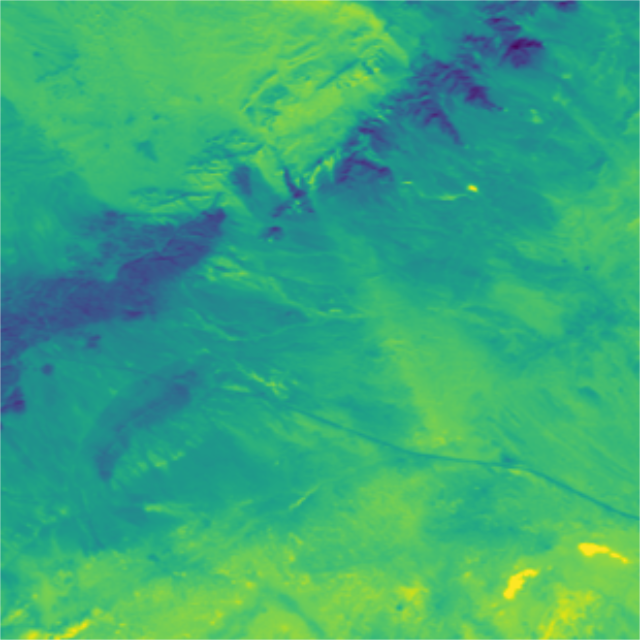
\includegraphics[width=\textwidth]{intermediate_hr}
        \caption{High--resolution}
    \end{subfigure}
    \hfill
    \centering
    \begin{subfigure}[t]{0.45\textwidth}
        \centering
        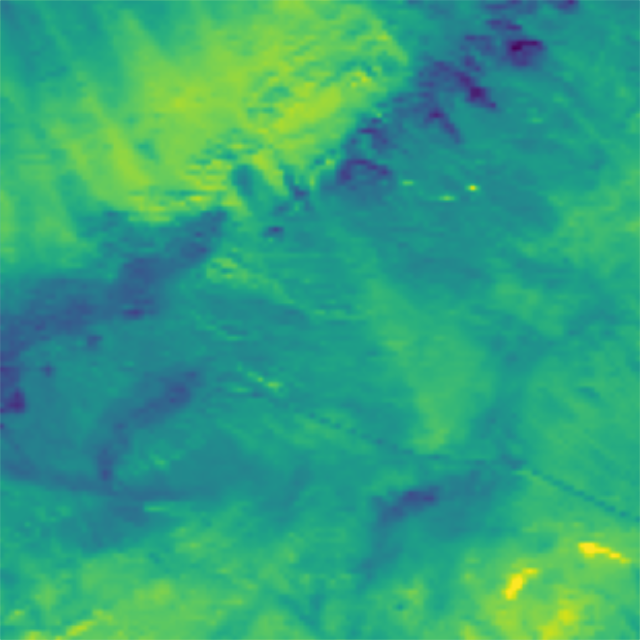
\includegraphics[width=\textwidth]{intermediate_lr}
        \caption{Low--resolution}
    \end{subfigure}
    \vskip\baselineskip
    \begin{subfigure}[t]{0.45\textwidth}
        \centering
        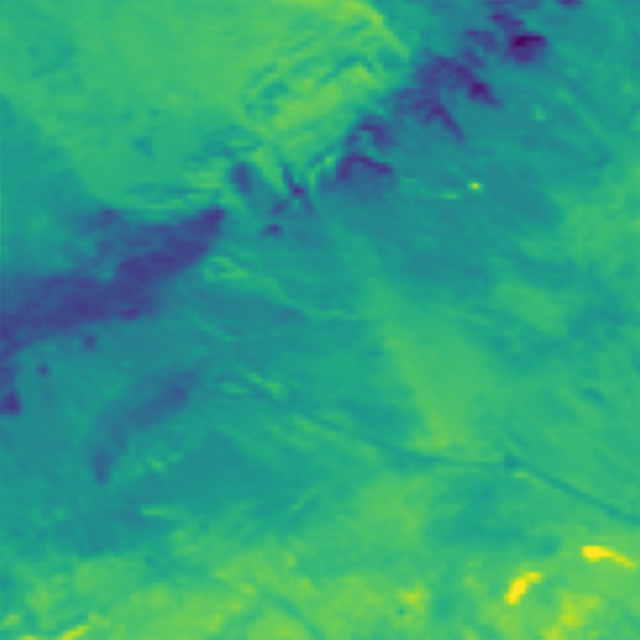
\includegraphics[width=\textwidth]{intermediate_lr_pred}
        \caption{Low--resolution augmented}
    \end{subfigure}
    \hfill
    \begin{subfigure}[t]{0.45\textwidth}
        \centering
        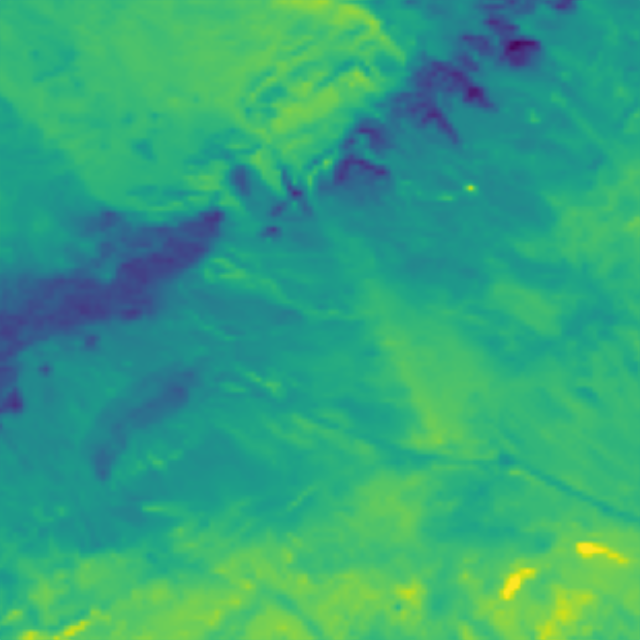
\includegraphics[width=\textwidth]{intermediate_lr_bicubic}
        \caption{Low resolution resized with bicubic}
    \end{subfigure}
    \caption{Intermediate results of evaluation on Proba--V test dataset for simple convolutional augmentation network}
    \label{fig:intermediate-results}
\end{figure}
\begin{figure}
    \begin{subfigure}[t]{0.45\textwidth}
        \centering
        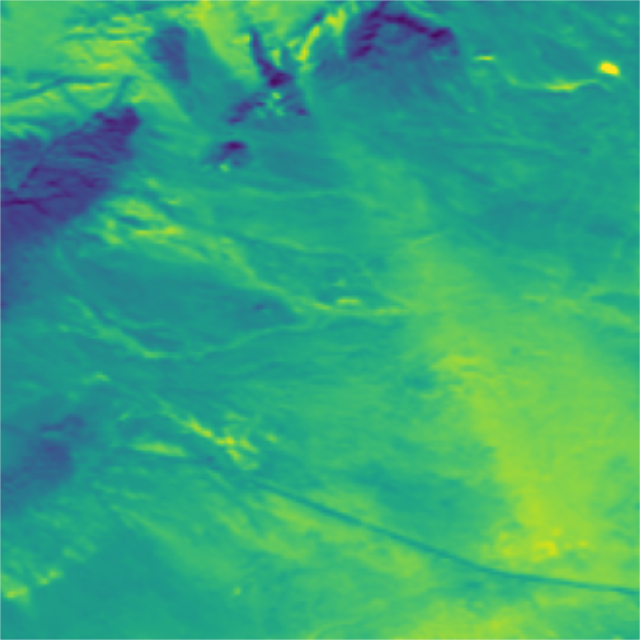
\includegraphics[width=\textwidth]{intermediate_zoomed_hr}
        \caption{High--resolution}
    \end{subfigure}
    \hfill
    \centering
    \begin{subfigure}[t]{0.45\textwidth}
        \centering
        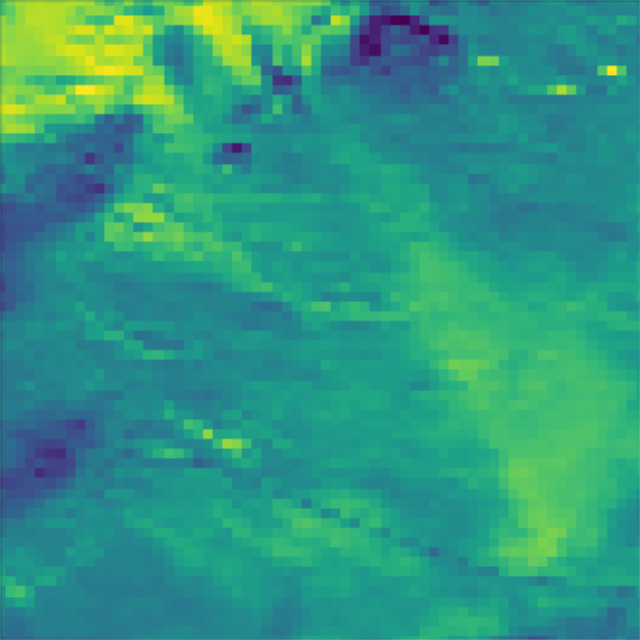
\includegraphics[width=\textwidth]{intermediate_zoomed_lr}
        \caption{Low--resolution}
    \end{subfigure}
    \vskip\baselineskip
    \begin{subfigure}[t]{0.45\textwidth}
        \centering
        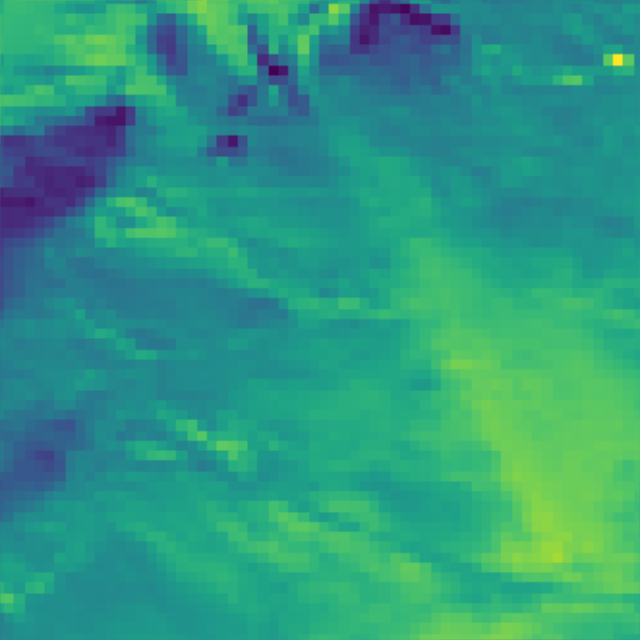
\includegraphics[width=\textwidth]{intermediate_zoomed_lr_pred}
        \caption{Low--resolution augmented}
    \end{subfigure}
    \hfill
    \begin{subfigure}[t]{0.45\textwidth}
        \centering
        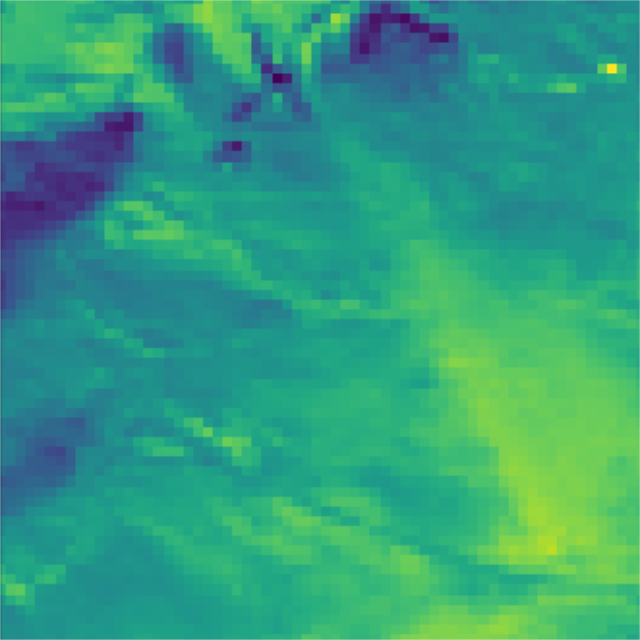
\includegraphics[width=\textwidth]{intermediate_zoomed_lr_bicubic}
        \caption{Low resolution resized with bicubic}
    \end{subfigure}
    \caption{Zoomed intermediate results of evaluation on Proba--V test dataset for simple convolutional augmentation network}
    \label{fig:intermediate-results-zoomed}
\end{figure}

The intermediate results indicate that the augmentation process works reasonably well and can be used for creating new datasets.
The numeric metrics look fairly similar for all given methods, their usefulness is to be determined during super--resolution training and evaluation.
Visual results also look well, low--resolution images resemble high--resolution ones.

\section{Implementation details}
As stated before, all networks were implemented in \textit{Python} using \textit{Tensorflow 2} library.
The built--in Keras interface offers several ways of building models; the most flexible one is called \textit{model subclassing}.
This approach enables using binary masks during training, thanks to possibility to overwrite the fitting method.
A custom train step with masking capability is shown in the listing \ref{lst:train_step_masking}.
\begin{listing}
\begin{minted}{python}
def train_step(self, data):
    x, y, y_mask = data

    with tf.GradientTape() as tape:
        y_pred = self(x, training=True)
        if self._use_lr_masks:
            y_pred = tf.boolean_mask(y_pred, y_mask)
            y = tf.boolean_mask(y, y_mask)
        loss = self.compiled_loss(
            y, y_pred, regularization_losses=self.losses)

    trainable_vars = self.trainable_variables
    gradients = tape.gradient(loss, trainable_vars)
    self.optimizer.apply_gradients(zip(gradients, trainable_vars))
    self.compiled_metrics.update_state(y, y_pred)
        return {m.name: m.result() for m in self.metrics}
\end{minted}
\caption{Custom train step method with masking capabilites}
\label{lst:train_step_masking}
\end{listing}


Model subclassing involves inheritance to implement custom training loops for Tensorflow models.
The simple convolutional and endcoder--decoder networks utilize this kind of model instantiation.
The GAN model uses a mixture of subclassing and \textit{Sequential API} which defines the model in a declarative way.
The two components of GAN---the generator and the discriminator are instantiated using the sequential approach, then they are combined into one using model subclassing.
A custom inference preview callback was implemented to enhance the training process.
Every training epoch a preview of inference on validation data is saved to a file.

\textit{Tensorboard} is a package accompanying Tensorflow that provides a convenient interface for training supervision.
It runs as a web server that displays a web page with the live progress of training in the form of interactive plots.
Tensorboard data is created using Keras' callbacks.
Callbacks are functions hooks called during specific steps of training.
They can provide features like previously discussed early stopping.
\textit{Model checkpoint} is another useful callback that saves the model at the end of the training epoch.
Tensorflow provides an interface for creating custom callbacks.
An inference preview mechanism on validation image at the end of each epoch was implemented as a custom callback.
This mechanism is very convenient when training the \textsc{gan} network.
Keras also enables writing custom losses and metrics.
This possibility has been used to write training losses based on PSNR and SSIM.
Both of them are based on internal Tensorflow implementations that were adjusted to serve as loss functions.

\chapter{Super--resolution training and evaluation}
\label{ch:sr-evaluation}
This chapter covers the training and evaluation of the HighRes-net super-resolution network trained with different datasets.
Various training possibilities are explored in regard to the network generalization problem.
The end of the chapter presents and discusses the summarized results.

\section{Training HighRes-net}
As stated in the experiment layout, the final step consists in training HighRes-net super-resolution model with different data.
One final step before conducting the training is to examine visually the results of augmentation on a Sentinel-2 image.
These are presented for the all the augmentation network architectures in Figures \ref{fig:export-example} and \ref{fig:export-example-zoomed}.
\begin{figure}
    \begin{subfigure}[t]{0.3\textwidth}
        \centering
        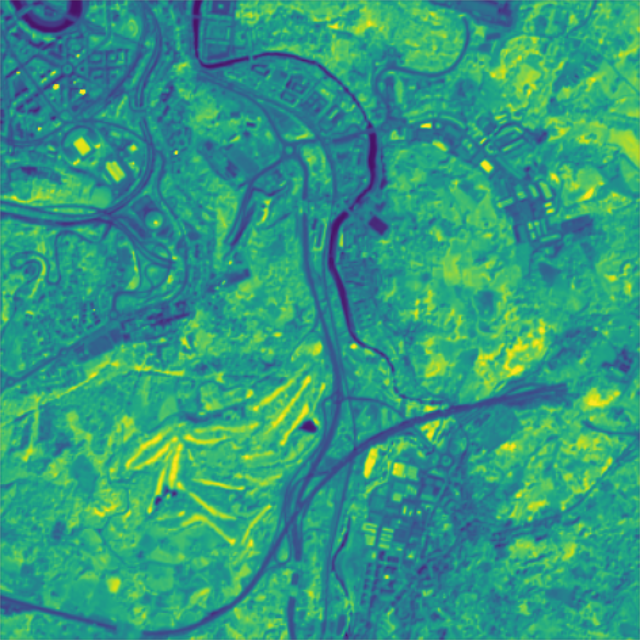
\includegraphics[width=\textwidth]{sentinel_export_hr}
        \caption{High-resolution}
    \end{subfigure}
    \hfill
    \begin{subfigure}[t]{0.3\textwidth}
        \centering
        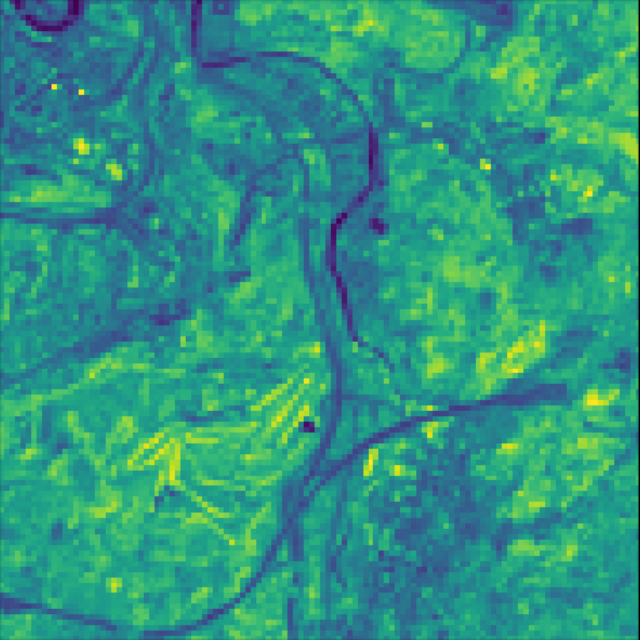
\includegraphics[width=\textwidth]{sentinel_export_bicubic}
        \caption{Low-resolution image created from the high-resolution one with bicubic interpolation}
    \end{subfigure}
    \hfill
    \begin{subfigure}[t]{0.3\textwidth}
        \centering
        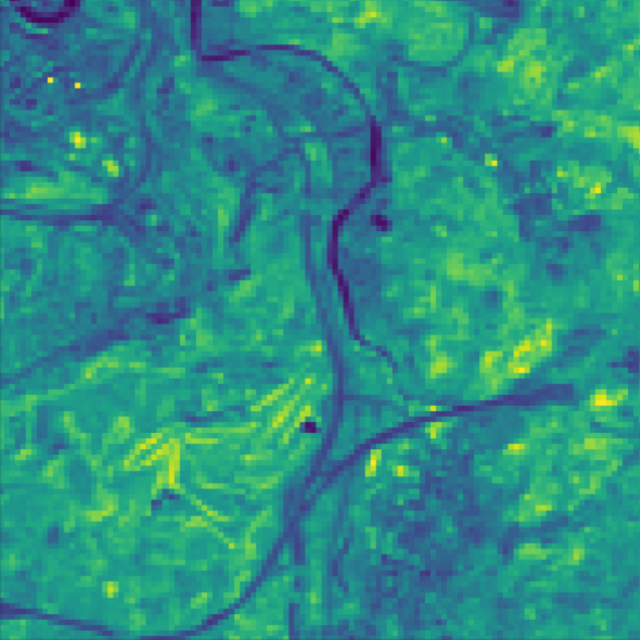
\includegraphics[width=\textwidth]{sentinel_export_simple_conv}
        \caption{Low-resolution image created from the high-resolution one by the simple convolutional network}
    \end{subfigure}
    \hfill
    \medskip
    \centering
    \hfill
    \begin{subfigure}[t]{0.3\textwidth}
        \centering
        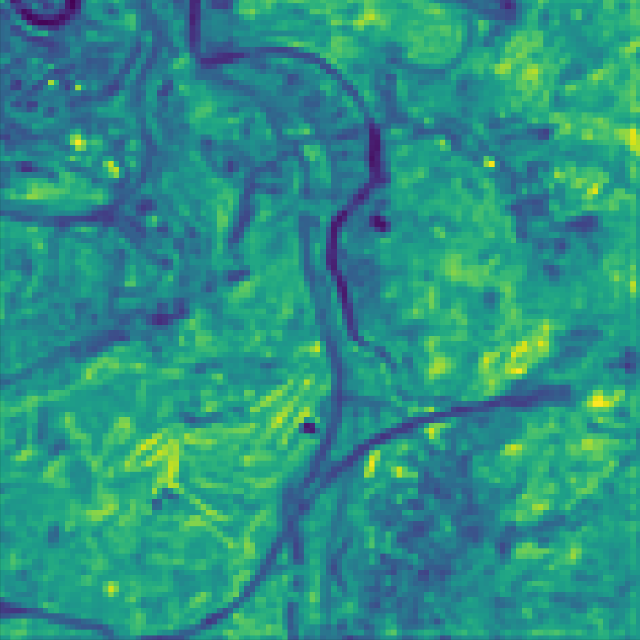
\includegraphics[width=\textwidth]{sentinel_export_autoencoder}
        \caption{Low-resolution image created from the high-resolution one by the encoder-decoder network}
    \end{subfigure}
    \quad
    \begin{subfigure}[t]{0.3\textwidth}
        \centering
        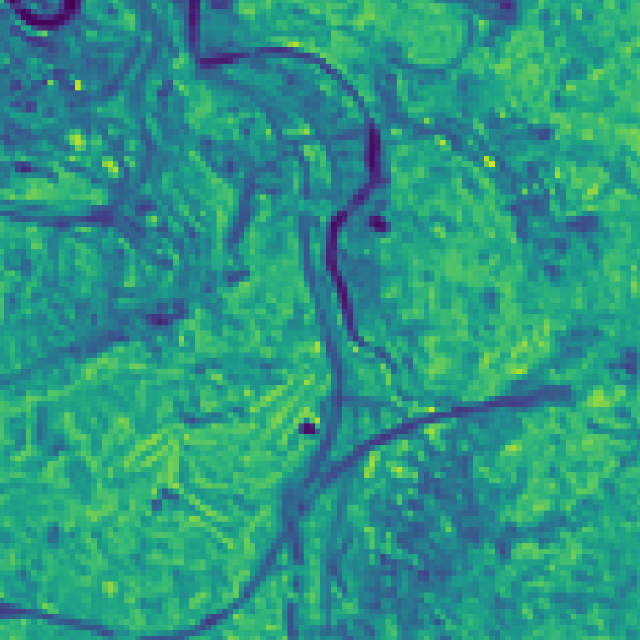
\includegraphics[width=\textwidth]{sentinel_export_gan}
        \caption{Low-resolution image created from the high-resolution one by the \gls{gan} network}
    \end{subfigure}
    \hfill
    \caption{Example of Sentinel-2 training dataset images created in different ways}
    \label{fig:export-example}
\end{figure}
\begin{figure}
        \begin{subfigure}[t]{0.3\textwidth}
        \centering
        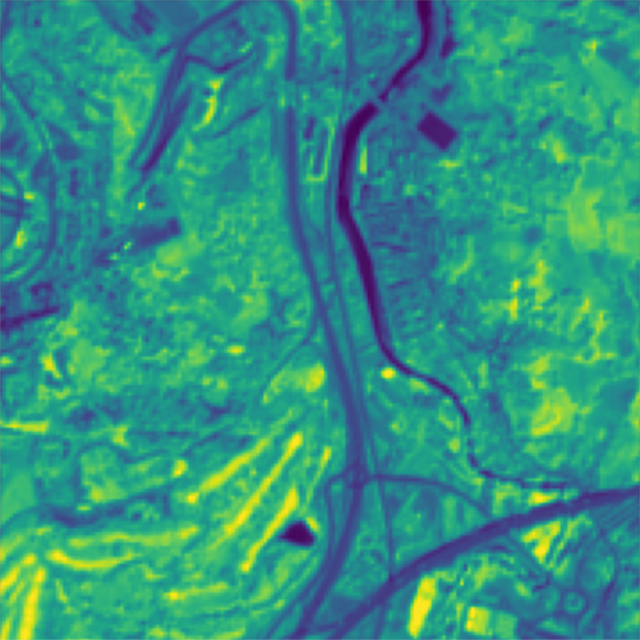
\includegraphics[width=\textwidth]{sentinel_export_zoomed_hr}
        \caption{High-resolution}
    \end{subfigure}
    \hfill
    \begin{subfigure}[t]{0.3\textwidth}
        \centering
        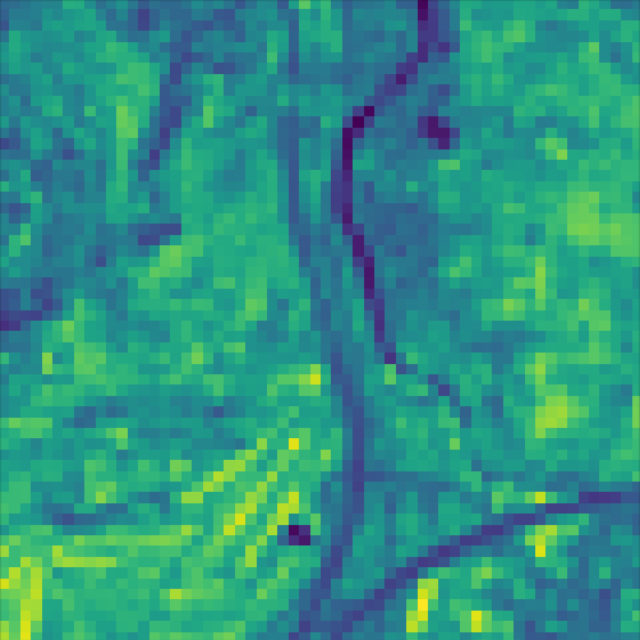
\includegraphics[width=\textwidth]{sentinel_export_zoomed_bicubic}
        \caption{Low-resolution image created from the high-resolution one with bicubic interpolation}
    \end{subfigure}
    \hfill
    \begin{subfigure}[t]{0.3\textwidth}
        \centering
        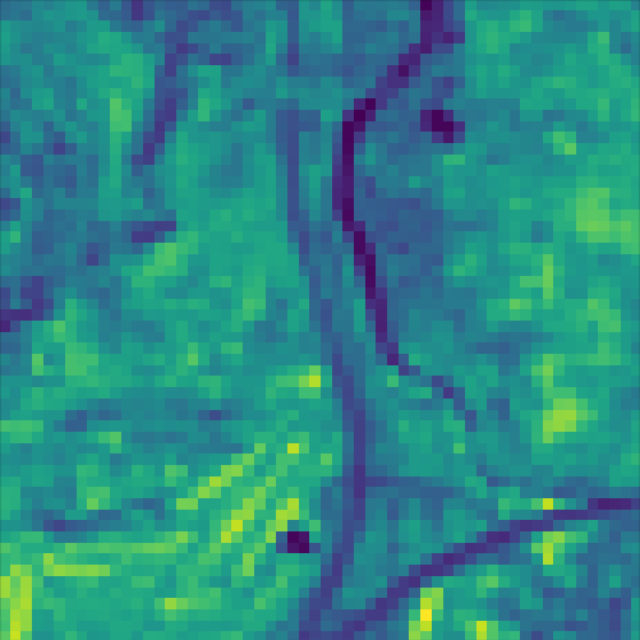
\includegraphics[width=\textwidth]{sentinel_export_zoomed_simple_conv}
        \caption{Low-resolution image created from the high-resolution one by the simple convolutional network}
    \end{subfigure}
    \hfill
    \medskip
    \centering
    \hfill
    \begin{subfigure}[t]{0.3\textwidth}
        \centering
        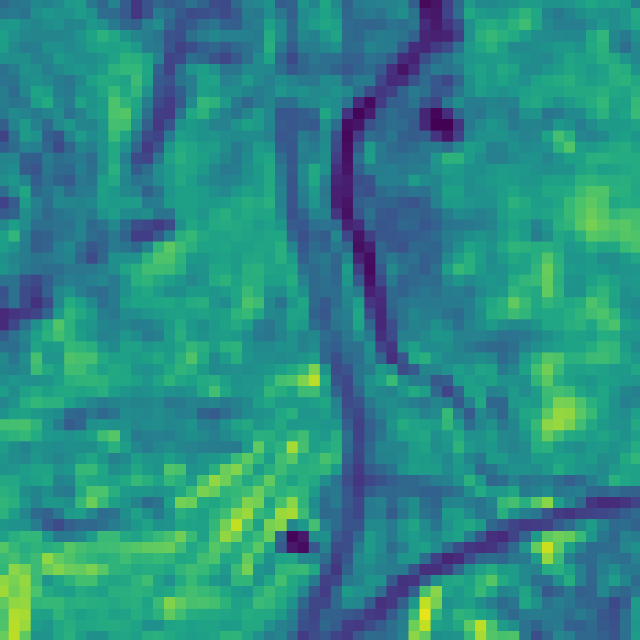
\includegraphics[width=\textwidth]{sentinel_export_zoomed_autoencoder}
        \caption{Low-resolution image created from the high-resolution one by the encoder-decoder network}
    \end{subfigure}
    \quad
    \begin{subfigure}[t]{0.3\textwidth}
        \centering
        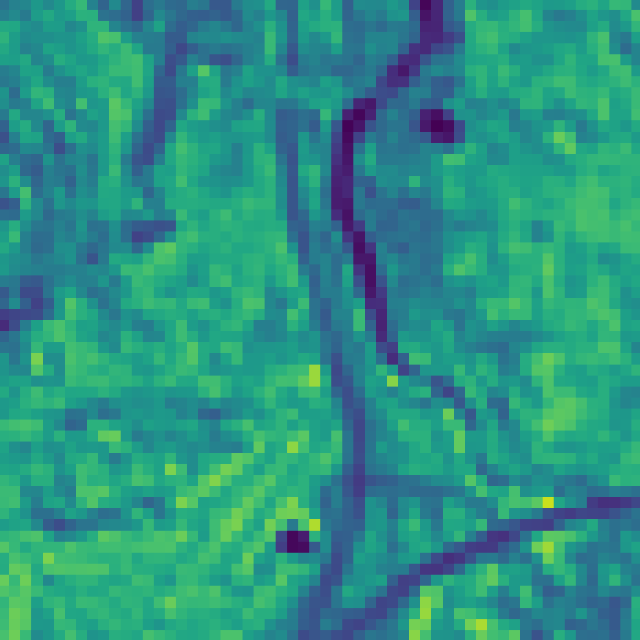
\includegraphics[width=\textwidth]{sentinel_export_zoomed_gan}
        \caption{Low-resolution image created from the high-resolution one by the \gls{gan} network}
    \end{subfigure}
    \hfill
    \caption{Zoomed examples of Sentinel-2 training dataset images created in different ways}
    \label{fig:export-example-zoomed}
\end{figure}

It should be kept in mind, that the training dataset created by resizing with bicubic interpolation was subject to additional transformations of contrast, noise, and blur as stated in Chapter \ref{ch:scope}.

As planned, the super-resolution is to be trained with multi-image data in a single-band (band eight) mode.
Training is configured in such a way that only weights for the best validation score are saved.
However, automatic stopping is not enabled.
For this reason, fitting was interrupted manually around epoch 100 when all training curves plateaued.
The training history has been plotted to visualize the fitting progress.
Figure \ref{fig:highres-net-training-loss} shows the loss history for all discussed HighRes-net trainings, Figure \ref{fig:highres-net-training-validation} presents the validation loss improvement.
Section \ref{sec:cross-type} discusses some parts of these figures in a more detailed way. 

\subsection{Stop condition based on cross-data-type validation}
\label{sec:cross-type}
Having multiple datasets generated in different ways enables an alternative way of validating the super-resolution training process.
Instead of taking a subpart of the training set as validation data, one may use images generated in a different way.
Such a technique may help to investigate the generalization capabilities of the super-resolution network.
This kind of validation is available thanks to the multiplicity of the generated datasets and is unique to this work.
The dataset created using the simple convolutional network and resizing algorithm were used for the cros-type-validation.
In this scheme the training and validation sets are created in different ways which enables broader look on evaluation during training.
It should be noticed, that the validation subsets were taken from the training datasets and not the evaluation test sets to prevent data leaks.
In Figures \ref{fig:highres-net-training-loss} and \ref{fig:highres-net-training-validation}, in the case of the cross-data-type validation scheme, the letter \textit{t} denotes the training dataset and the letter \textit{v} denotes the validation dataset.
When using the cross-data-type evaluation the validation loss stops to decrease significantly earlier, as seen in Figure \ref{fig:highres-net-training-validation}.
A small raise in validation loss is visible for over ten epochs before the training was stopped.
In this case, the best weights were saved nearly three times earlier than during the non-cross-type-validated training. 
This may indicate that the vast part of the fitting process does not contribute to the overall generalization capability of the super-resolution network.
The cross-validated training is stopped earlier; since only weights for the epoch with the best validation score are saved, it is pointless to run longer fittings.
\begin{figure}
    \centering
    \begin{tikzpicture}
			\begin{axis}[width=\linewidth, height=12cm, xmin=-9.9, xmax=110, legend cell align={left}, ymode=log, grid=major, grid style={dashed}, xlabel=Epoch, ylabel=Loss]
			\addlegendentry{Bicubic}
			\addplot+[mark=none] table [x=step, y=value, col sep=comma] {data/highresnet_s2ab_ab5_bb8_20210608-114450-training_loss.csv};
			\addlegendentry{Simple convolutional}
						\addplot+[mark=none] table [x=step, y=value, col sep=comma] {data/highresnet_s2_degraded_simple_conv-dvc-21-07-04_044726_e34_bb8_20210706-183639-training_loss.csv};
			\addlegendentry{Encoder-decoder}
						\addplot+[mark=none] table [x=step, y=value, col sep=comma] {data/highresnet_s2_degraded_autoencoder-dvc-21-07-04-052647_e23_bb8_20210707-100146-training_loss.csv};
			\addlegendentry{\gls{gan}}
						\addplot+[mark=none] table [x=step, y=value, col sep=comma] {data/highresnet_s2_degraded-gan-dvc-21-07-04-055506_e94_bb8_20210707-152641-training_loss.csv};
			\addlegendentry{t: Bicubic, v: Simple convolutional}
						\addplot+[mark=none, color=green] table [x=step, y=value, col sep=comma] {data/highresnet_s2ab_ab5_bb8_20210726-160215-training_loss.csv};

			\end{axis}		\end{tikzpicture}
    \caption{HighRes-net training loss history with training sets created in different ways}
    \label{fig:highres-net-training-loss}
\end{figure}
\begin{figure}
    \centering
    \begin{tikzpicture}
			\begin{axis}[width=\linewidth, height=12cm, xmin=-9.9, xmax=110, legend cell align={left}, grid=major, grid style={dashed}, xlabel=Epoch, ylabel=Loss]
			\addlegendentry{Bicubic}
			\addplot+[mark=none] table [x=step, y=value, col sep=comma] {data/highresnet_s2ab_ab5_bb8_20210608-114450-validation_loss.csv};
			\addlegendentry{Simple convolutional}
						\addplot+[mark=none] table [x=step, y=value, col sep=comma] {data/highresnet_s2_degraded_simple_conv-dvc-21-07-04_044726_e34_bb8_20210706-183639-validation_loss.csv};
			\addlegendentry{Encoder-decoder}
						\addplot+[mark=none] table [x=step, y=value, col sep=comma] {data/highresnet_s2_degraded_autoencoder-dvc-21-07-04-052647_e23_bb8_20210707-100146-validation_loss.csv};
			\addlegendentry{\gls{gan}}
						\addplot+[mark=none] table [x=step, y=value, col sep=comma] {data/highresnet_s2_degraded-gan-dvc-21-07-04-055506_e94_bb8_20210707-152641-validation_loss.csv};
			\addlegendentry{t: Bicubic, v: Simple convolutional}
						\addplot+[mark=none, color=green] table [x=step, y=value, col sep=comma] {data/highresnet_s2ab_ab5_bb8_20210726-160215-validation_loss.csv};

			\end{axis}		\end{tikzpicture}
    \caption{HighRes-net validation loss history with training sets created in different ways}
    \label{fig:highres-net-training-validation}
\end{figure}

\section{Evaluation and results}
According to the experiment layout, the trained super-resolution models are to be evaluated on a variety of test datasets to examine generalization capabilities and robustness.
As stated before, the evaluation datasets include:
\begin{itemize}
	\item Test subsets from all augmented Sentinel-2 datasets that can be used for calculating numerical metrics.
	\item Real-life Sentinel-2 images that were not used in the training process and do not include high and low-resolution pairs, so only visual examination can be performed. These are original images that were not downsampled. This means that they have different resolution and \gls{gsd} than the low-resolution images in the artificial datasets used for training the super-resolution networks. 
	\item Proba-V original real-life test dataset that can be used for calculating numerical metrics.
\end{itemize}
It should be noticed, that the latter two test sets differ in the \gls{gsd} parameter from the synthetic low-resolution images in the Sentinel-2 training datasets.
This data is still valid for evaluation and investigation because it is desirable that super-resolution and machine learning algorithms in general work on objects of any scale and size.
Limiting the tests to a single \gls{gsd} would draw an incomplete picture of the results.
The results of the evaluation are presented in Table \ref{tab:super-res-results}, where rows designate test datasets and columns indicate models trained on data created in different ways.
For the cross-validation training scenarios, letters \textit{t} and \textit{v} indicate the training and validation datasets respectively.
The cPSNR score was used as the super-resolution evaluation metric.

The best results are observed along the diagonal of the table, which means that the super-resolution model works best on test data created in the same way as training data for a given model.
A visual demonstration of such an evaluation can be seen in Figure \ref{fig:highresnet-test-visual}.
In this case, HighRes-net was trained on the dataset created by the simple convolutional network and evaluated on the test subpart of the same dataset.
An example of image upscaling with bicubic interpolation was included in the figure as a reference point.
The best results along the diagonal are expected and indicate that no gross mistakes were made in the course of the work.
Each network works best on the data created in the same way as its training set.
The super-resolution network trained using data generated by the simple convolutional network recreates the original high-resolution images best (with cPSNR of 36.15).
\begin{figure}
    \centering
    \begin{subfigure}[t]{0.45\textwidth}
        \centering
        
\includegraphics[width=\textwidth]{highresnet_test_lr}
        \caption{One of nine low-resolution images}
    \end{subfigure}
    \hfill
    \begin{subfigure}[t]{0.45\textwidth}
        \centering
        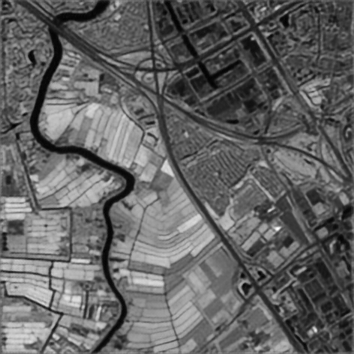
\includegraphics[width=\textwidth]{highresnet_test_sr}
        \caption{Super-resolution reconstruction of the scene}
    \end{subfigure}
    \begin{subfigure}[t]{0.45\textwidth}
        \centering
        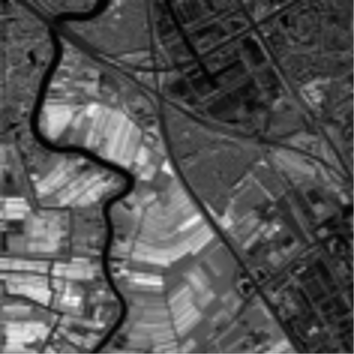
\includegraphics[width=\textwidth]{highresnet_test_bicubic}
        \caption{Upscaling to high-resolution with bicubic interpolation}
    \end{subfigure}
    \hfill
    \begin{subfigure}[t]{0.45\textwidth}
        \centering
        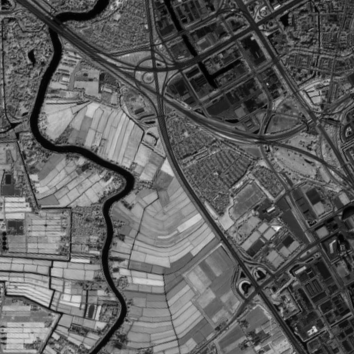
\includegraphics[width=\textwidth]{highresnet_test_hr}
        \caption{Real-life high-resolution picture of the scene}
    \end{subfigure}
    \caption{A visual example of evaluation of an augmented dataset; both the training and test datasets were generated using the simple convolutional network}
    \label{fig:highresnet-test-visual}
\end{figure}
\begin{table}
\caption{Evaluation of super-resolution training on different test sets (cPSNR metric, the larger, the better)}
\label{tab:super-res-results}
\begin{adjustbox}{center}
\small
\begin{tabular}{@{}llccccc@{}}
\toprule
\multicolumn{2}{c}{\multirow{2}{*}{}} & \multicolumn{5}{c}{\textbf{Training data}}                                             \\ \cmidrule{3-7} 
\multicolumn{2}{c}{} &
  Bicubic &
  Simple conv &
  Encoder-decoder &
  \gls{gan} &
  \begin{tabular}[c]{@{}c@{}}t: Bicubic\\ v: Simple conv\end{tabular} \\ \midrule
\multirow{5}{*}{\rotatebox[origin=c]{90}{\textbf{Test data}}} &
  Bicubic &
  \textbf{35.78} &
  28.96 &
  24.55 &
  25.80 &
  35.26 \\
           & Simple conv          & 33.69 & \textbf{36.15} & 27.16          & 29.83          & 33.67          \\
           & Encoder-decoder               & 31.72 & 31.78          & \textbf{34.43} & 30.22          & 31.76          \\
           & \gls{gan}                     & 28.63 & 28.63          & 27.27          & \textbf{35.72} & 30.28          \\
           & Proba-V                       & 43.36 & 42.02          & 40.43          & 40.91          & \textbf{43.51} \\ \bottomrule
\end{tabular}
\end{adjustbox}
\end{table}

As stated in Chapter \ref{ch:scope}, an additional set of original real-life Sentinel-2 images is available.
This set includes single-resolution images with different \gls{gsd} than the synthetic training datasets.
Since this set does not feature high and low-resolution image pairs, it can be used only for visual examination.
Samples for such visual evaluation are shown in Figure \ref{fig:sentinel-real-artifacts}.
Some mosaic or checkerboard-like artifacts can be observed in the super-resolved images.
As seen in the samples, some form of artifacts occurred for all the networks on real-life Sentinel-2 data (with higher \gls{gsd} than the training low-resolution images).
\begin{figure}
    \centering
    \begin{subfigure}[t]{0.32\textwidth}
        \centering
        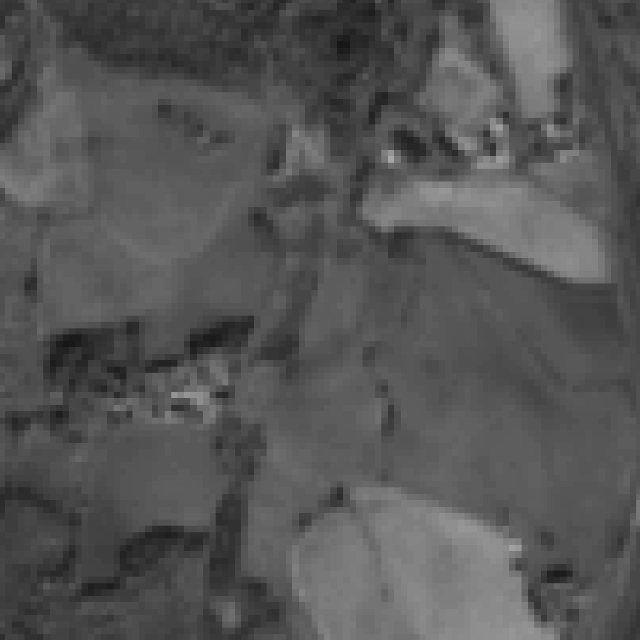
\includegraphics[width=\textwidth]{sentinel_real_lr}
        \caption{One of the low-resolution images of the test scene}
    \end{subfigure}
    \hfill
    \begin{subfigure}[t]{0.32\textwidth}
        \centering
        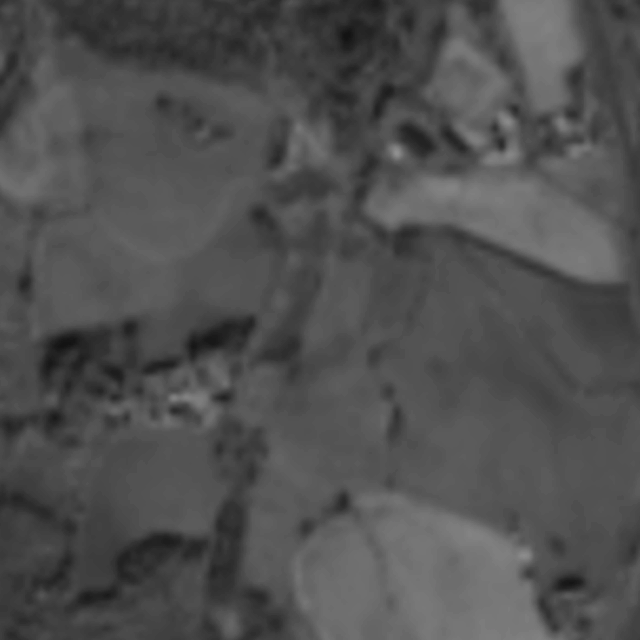
\includegraphics[width=\textwidth]{sentinel_real_upscale_bicubic} 
        \caption{Upscaling to high-resolution with bicubic interpolation}
    \end{subfigure}
    \hfill
    \begin{subfigure}[t]{0.32\textwidth}
        \centering
        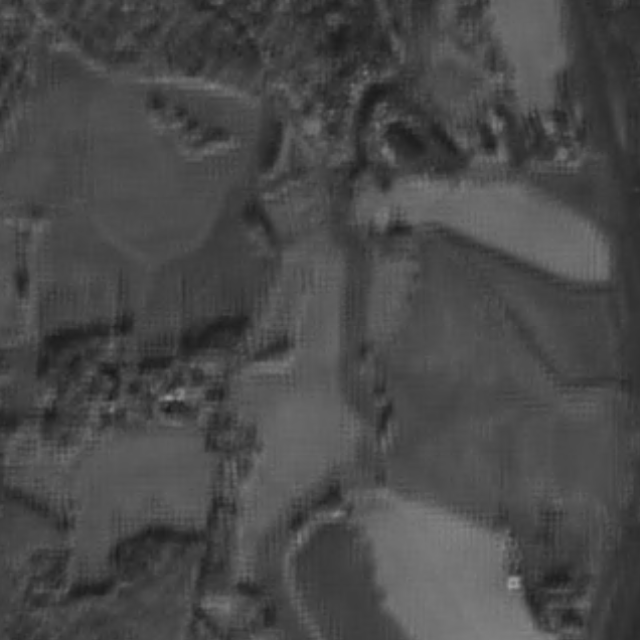
\includegraphics[width=\textwidth]{setinel_real_sr_bicubic}
        \caption{HigRes-net trained on data created with bicubic interpolation}
    \end{subfigure}
    \hfill
    \smallskip
    \centering
    \hfill
    \begin{subfigure}[t]{0.32\textwidth}
        \centering
        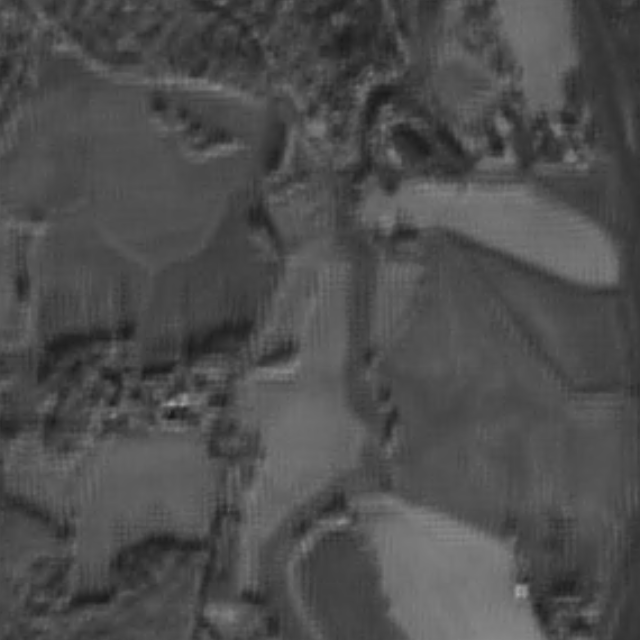
\includegraphics[width=\textwidth]{sentinel_real_sr_simple_tbic_vsimple}
        \caption{HigRes-net trained on data created with bicubic interpolation; training done with cross-data-type validation}
    \end{subfigure}
    \hfill
    \begin{subfigure}[t]{0.32\textwidth}
        \centering
         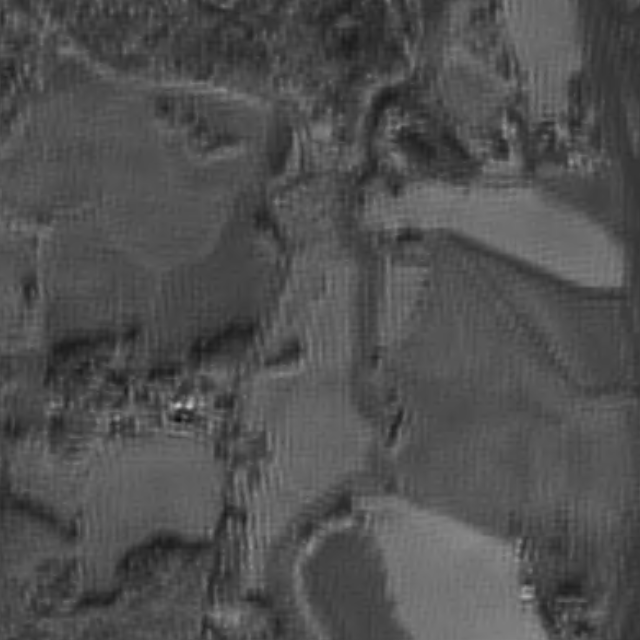
\includegraphics[width=\textwidth]{sentinel_real_sr_simple_conv}
        \caption{HigRes-net trained on data created by the simple conv network}
    \end{subfigure}
    \hfill
    \begin{subfigure}[t]{0.32\textwidth}
        \centering
        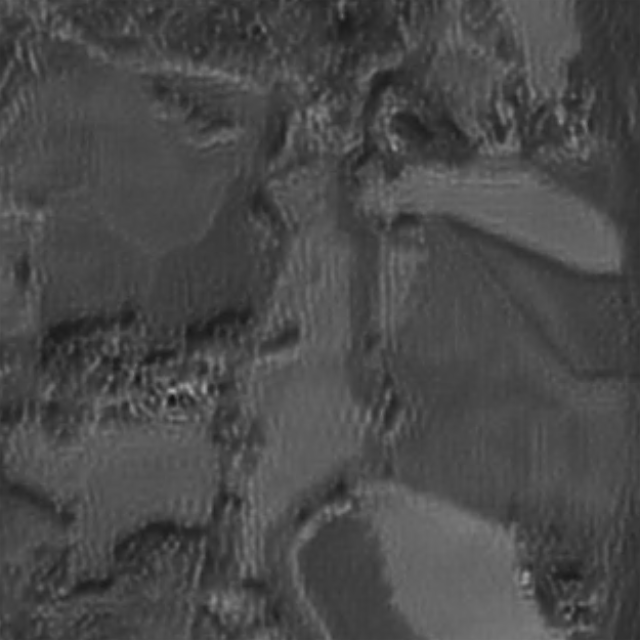
\includegraphics[width=\textwidth]{sentinel_real_sr_autoencoder}
        \caption{HigRes-net trained on data created by the encoder-decoder network}
    \end{subfigure}
    \hfill
    \smallskip
    \centering
    \hfill
    \begin{subfigure}[t]{0.32\textwidth}
        \centering
        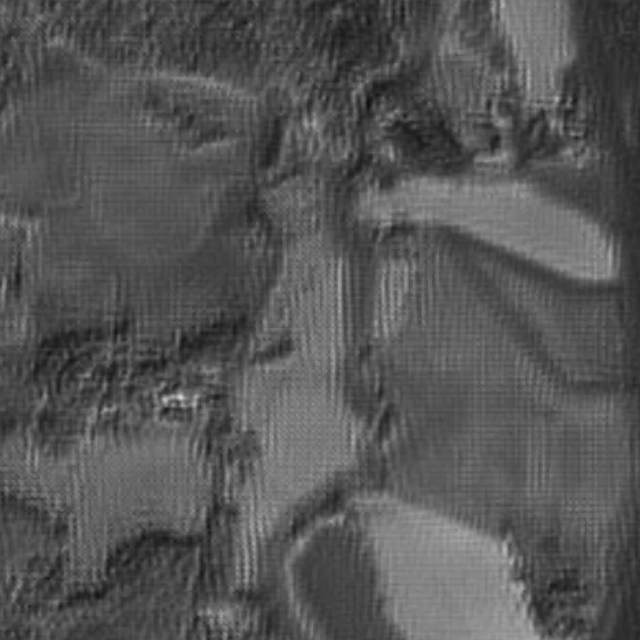
\includegraphics[width=\textwidth]{sentinel_real_sr_simple_gan}
        \caption{HigRes-net trained on data created by the \gls{gan} network}
    \end{subfigure}
    \hfill
    \captionsetup{justification=justified}
    \caption{A visual evaluation of super-resolution results on real-life Sentinel-2 test data. Images are super-resolved by HighRes-net trained on datasets created in different ways. One of the original low-resolution images and a high-resolution one created by upscaling with bicubic interpolation are added for reference.}
    \label{fig:sentinel-real-artifacts}
\end{figure}

The results in Table \ref{tab:super-res-results} and Figure \ref{fig:sentinel-real-artifacts} can be summarized in the following statements:
\begin{itemize}
	\item Data created with augmentation techniques, both traditional and deep learning-based is suitable for training super-resolution networks.
	\item The different deep learning architectures give fairly similar results, although the simplest one works best (achieves best results for the real-life Proba-V test subset).
	\item At the moment, the bicubic interpolation gives slightly better results for the real-life Proba-V test subset. Possible reasons for that and suggestions of improvement are included in the summary.
	\item The cross-data-type-validation proves that all trainings are prone to overfitting to the data generation techniques. Early stopping based on different datasets can lead to this conclusion. Using cross-data-type-validation resulted in a network that was trained for fewer epochs, yet performed slightly better on the real-life Proba-V test subset.
	\item The generalization capabilities of the networks trained on synthetic data pose a problem. Artifacts on real data can be observed.
\end{itemize}

\chapter{Summary}
\label{ch:summary}
In the course of the work various approach to data augmentation were explored.
Three different deep leaning architectures were introduced and compared with the traditional approach.
The augmentation networks were trained on real--life data and used to export new datasets to fit the super--resolution algorithm.
Then the super--resolution models were evaluated on various synthetic and real--file images; both in numerical and visual way.
The cross--validation based approach to training supervision proved to be valuable.
The deep learning based methods proved to be of utility, yet slightly below what would be expected, since they didn't surpass the bicubic interpolation approach.
There may be a variety of reasons for that to explore.
Many possibilities were not explored in a full way; translations between low--resolution images, may be investigated in a greater detail.
Modeling them after distribution extracted from a real--world dataset may lead to enhanced results.
The semi--simulated approach for data generation was not included in the scope of the work, however it would be interesting to investigate this option in the future.

The most novel observation in the work is connected with the cross--validation technique during training.
Early stopping training based on this approach lead to good results.
This indicates a greater overfitting problem in regard to data generation method.
The robust data augmentation problem remains open, however valuable observations about issue of super--resolution generalization has been made.

There is value in the opportunity for further development of the work and more detailed investigation.
Achieving robustness and greater generalization of super--resolution techniques through better data augmentation is an important step towards productization of this technique.
A super--resolution algorithm independent of satellite data type would be useful in image  processing pipeline during aerospace missions, remote sensing tasks and Earth observations.

\begin{appendices}
    \chapter{Model and training parameters of the augmentation networks}
\label{ch:appendix-params}
As stated in the work the models and training process are parametrized by set o variables in a \textit{params.yaml} file.
This file is supervised by Git and \gls{dvc} to ensure reproducibility and artifacts caching.
Contents of the configuration file during the training of augmentation networks are presented in Listing \ref{lst:params-file}.
\begin{longlisting}
\inputminted{yaml}{listings/params.yaml}
\caption{Contents of the \textit{params.yaml} file used for training}
\label{lst:params-file}
\end{longlisting}

\chapter{Technical documentation}
\label{ch:appendix-technical}
As mentioned in Section \ref{sec:exp-management} trainings are done either done with the aid of the \gls{dvc} system or by running scripts manually.
The trainings done automatically by the \gls{dvc} system contain the word \textit{dvc} as the experiment name.
The status of these trainings is supervised by \gls{dvc}, current progress can be checked with the \mintinline[breaklines]{shell}{dvc status} command.
Trainings are automatically rerun or recached based on configuration files after running the \mintinline[breaklines]{shell}{dvc repro} instruction.
Manual trainings are run by invoking Python directly.
This can be done with the command: \mintinline[breaklines]{shell}{python -m cnn_res_degrader.train [-s] [-a] [-g] training_name} where the optional arguments decide which architecture to train and the positional argument is the experiment name.

Validation on Proba-V dataset can be run with the command: \mintinline[breaklines]{shell}{python -m cnn_res_degrader.test [-s|-a|-g] weights_path output_dir} where the positional stores model architecture and positional arguments hold paths to trained model weights and output directory.

The augmented Sentinel-2 datasets can be created by running the command: \mintinline[breaklines]{shell}{python -m export_sentinel.py [-s|-a|-g] [-r] [-d] weights_path}, where architecture and path to weights are denoted as described earlier.
The last two of the switches enable generating random translations (instead of using ones saved in sentinel files) and running a demo export on one image (instead of using the whole dataset).

\chapter{Supplementary media}
The supplementary media include:
\begin{itemize}
	\item This document.
	\item Source code files.
	\item The datasets can be fetched from the cloud using \gls{dvc}; to gain access to the data contact the author for the passcodes.
\end{itemize}

\end{appendices}

% Lists of objects
\listoffigures
\listoftables
\listofalgorithms
\listoflistings

% Bibliography
\nocite{*}
\bibliographystyle{plplain}
\bibliography{references}

\end{document}
